\documentclass[twoside]{book}

% Packages required by doxygen
\usepackage{fixltx2e}
\usepackage{calc}
\usepackage{doxygen}
\usepackage[export]{adjustbox} % also loads graphicx
\usepackage{graphicx}
\usepackage[utf8]{inputenc}
\usepackage{makeidx}
\usepackage{multicol}
\usepackage{multirow}
\PassOptionsToPackage{warn}{textcomp}
\usepackage{textcomp}
\usepackage[nointegrals]{wasysym}
\usepackage[table]{xcolor}

% Font selection
\usepackage[T1]{fontenc}
\usepackage[scaled=.90]{helvet}
\usepackage{courier}
\usepackage{amssymb}
\usepackage{sectsty}
\renewcommand{\familydefault}{\sfdefault}
\allsectionsfont{%
  \fontseries{bc}\selectfont%
  \color{darkgray}%
}
\renewcommand{\DoxyLabelFont}{%
  \fontseries{bc}\selectfont%
  \color{darkgray}%
}
\newcommand{\+}{\discretionary{\mbox{\scriptsize$\hookleftarrow$}}{}{}}

% Page & text layout
\usepackage{geometry}
\geometry{%
  a4paper,%
  top=2.5cm,%
  bottom=2.5cm,%
  left=2.5cm,%
  right=2.5cm%
}
\tolerance=750
\hfuzz=15pt
\hbadness=750
\setlength{\emergencystretch}{15pt}
\setlength{\parindent}{0cm}
\setlength{\parskip}{3ex plus 2ex minus 2ex}
\makeatletter
\renewcommand{\paragraph}{%
  \@startsection{paragraph}{4}{0ex}{-1.0ex}{1.0ex}{%
    \normalfont\normalsize\bfseries\SS@parafont%
  }%
}
\renewcommand{\subparagraph}{%
  \@startsection{subparagraph}{5}{0ex}{-1.0ex}{1.0ex}{%
    \normalfont\normalsize\bfseries\SS@subparafont%
  }%
}
\makeatother

% Headers & footers
\usepackage{fancyhdr}
\pagestyle{fancyplain}
\fancyhead[LE]{\fancyplain{}{\bfseries\thepage}}
\fancyhead[CE]{\fancyplain{}{}}
\fancyhead[RE]{\fancyplain{}{\bfseries\leftmark}}
\fancyhead[LO]{\fancyplain{}{\bfseries\rightmark}}
\fancyhead[CO]{\fancyplain{}{}}
\fancyhead[RO]{\fancyplain{}{\bfseries\thepage}}
\fancyfoot[LE]{\fancyplain{}{}}
\fancyfoot[CE]{\fancyplain{}{}}
\fancyfoot[RE]{\fancyplain{}{\bfseries\scriptsize Generated by Doxygen }}
\fancyfoot[LO]{\fancyplain{}{\bfseries\scriptsize Generated by Doxygen }}
\fancyfoot[CO]{\fancyplain{}{}}
\fancyfoot[RO]{\fancyplain{}{}}
\renewcommand{\footrulewidth}{0.4pt}
\renewcommand{\chaptermark}[1]{%
  \markboth{#1}{}%
}
\renewcommand{\sectionmark}[1]{%
  \markright{\thesection\ #1}%
}

% Indices & bibliography
\usepackage{natbib}
\usepackage[titles]{tocloft}
\setcounter{tocdepth}{3}
\setcounter{secnumdepth}{5}
\makeindex

% Hyperlinks (required, but should be loaded last)
\usepackage{ifpdf}
\ifpdf
  \usepackage[pdftex,pagebackref=true]{hyperref}
\else
  \usepackage[ps2pdf,pagebackref=true]{hyperref}
\fi
\hypersetup{%
  colorlinks=true,%
  linkcolor=blue,%
  citecolor=blue,%
  unicode%
}

% Custom commands
\newcommand{\clearemptydoublepage}{%
  \newpage{\pagestyle{empty}\cleardoublepage}%
}

\usepackage{caption}
\captionsetup{labelsep=space,justification=centering,font={bf},singlelinecheck=off,skip=4pt,position=top}

%===== C O N T E N T S =====

\begin{document}

% Titlepage & ToC
\hypersetup{pageanchor=false,
             bookmarksnumbered=true,
             pdfencoding=unicode
            }
\pagenumbering{alph}
\begin{titlepage}
\vspace*{7cm}
\begin{center}%
{\Large markets }\\
\vspace*{1cm}
{\large Generated by Doxygen 1.8.13}\\
\end{center}
\end{titlepage}
\clearemptydoublepage
\pagenumbering{roman}
\tableofcontents
\clearemptydoublepage
\pagenumbering{arabic}
\hypersetup{pageanchor=true}

%--- Begin generated contents ---
\chapter{Class Index}
\section{Class List}
Here are the classes, structs, unions and interfaces with brief descriptions\+:\begin{DoxyCompactList}
\item\contentsline{section}{\hyperlink{classbase__mod}{base\+\_\+mod} \\*Each model must inherit from this abstract base class }{\pageref{classbase__mod}}{}
\item\contentsline{section}{\hyperlink{classCSVReader}{C\+S\+V\+Reader} }{\pageref{classCSVReader}}{}
\item\contentsline{section}{\hyperlink{classDataHandler}{Data\+Handler} }{\pageref{classDataHandler}}{}
\item\contentsline{section}{\hyperlink{classExecHandler}{Exec\+Handler} }{\pageref{classExecHandler}}{}
\item\contentsline{section}{\hyperlink{classFill}{Fill} }{\pageref{classFill}}{}
\item\contentsline{section}{\hyperlink{classInstrument}{Instrument} }{\pageref{classInstrument}}{}
\item\contentsline{section}{\hyperlink{classMarketBar}{Market\+Bar} }{\pageref{classMarketBar}}{}
\item\contentsline{section}{\hyperlink{classMarketSnapshot}{Market\+Snapshot} }{\pageref{classMarketSnapshot}}{}
\item\contentsline{section}{\hyperlink{classMarketSnapshotsMaker}{Market\+Snapshots\+Maker} }{\pageref{classMarketSnapshotsMaker}}{}
\item\contentsline{section}{\hyperlink{classModelBank}{Model\+Bank} \\*Container of all your models }{\pageref{classModelBank}}{}
\item\contentsline{section}{\hyperlink{classMoveAve}{Move\+Ave} \\*Simple moving average class used to store the most recent model log-\/likelihoods }{\pageref{classMoveAve}}{}
\item\contentsline{section}{\hyperlink{classOrder}{Order} }{\pageref{classOrder}}{}
\item\contentsline{section}{\hyperlink{classpnl__calc}{pnl\+\_\+calc} }{\pageref{classpnl__calc}}{}
\item\contentsline{section}{\hyperlink{classPortfolio}{Portfolio} }{\pageref{classPortfolio}}{}
\item\contentsline{section}{\hyperlink{classPositionSummary}{Position\+Summary} }{\pageref{classPositionSummary}}{}
\end{DoxyCompactList}

\chapter{File Index}
\section{File List}
Here is a list of all files with brief descriptions\+:\begin{DoxyCompactList}
\item\contentsline{section}{include/\hyperlink{data__handlers_8h}{data\+\_\+handlers.\+h} \\*Helps convert \hyperlink{classMarketSnapshot}{Market\+Snapshot} events into Eigen\+::\+Vector\+Xds }{\pageref{data__handlers_8h}}{}
\item\contentsline{section}{include/\hyperlink{data__readers_8h}{data\+\_\+readers.\+h} \\*Reads in data (assumed in a certain format), and parses it into a vector of Market\+Snapshots }{\pageref{data__readers_8h}}{}
\item\contentsline{section}{include/\hyperlink{execution__handler_8h}{execution\+\_\+handler.\+h} }{\pageref{execution__handler_8h}}{}
\item\contentsline{section}{include/\hyperlink{fill_8h}{fill.\+h} }{\pageref{fill_8h}}{}
\item\contentsline{section}{include/\hyperlink{instrument_8h}{instrument.\+h} \\*Represents a tradable instrument in the financial markets }{\pageref{instrument_8h}}{}
\item\contentsline{section}{include/\hyperlink{market__bar_8h}{market\+\_\+bar.\+h} \\*Represents a summary of market data for a particular instrument over a given period of time }{\pageref{market__bar_8h}}{}
\item\contentsline{section}{include/\hyperlink{market__snapshot_8h}{market\+\_\+snapshot.\+h} \\*Represents a snapshot of the market at a particular point in time }{\pageref{market__snapshot_8h}}{}
\item\contentsline{section}{include/\hyperlink{model__bank_8h}{model\+\_\+bank.\+h} }{\pageref{model__bank_8h}}{}
\item\contentsline{section}{include/\hyperlink{order_8h}{order.\+h} \\*\hyperlink{classOrder}{Order} class with const public data members }{\pageref{order_8h}}{}
\item\contentsline{section}{include/\hyperlink{pnl__calculator_8h}{pnl\+\_\+calculator.\+h} }{\pageref{pnl__calculator_8h}}{}
\item\contentsline{section}{include/\hyperlink{portfolio_8h}{portfolio.\+h} \\*This represents the top level of all accounting details }{\pageref{portfolio_8h}}{}
\item\contentsline{section}{include/\hyperlink{position__summary_8h}{position\+\_\+summary.\+h} \\*Provides a collection of Position objects }{\pageref{position__summary_8h}}{}
\item\contentsline{section}{include/\hyperlink{run__backtest_8h}{run\+\_\+backtest.\+h} }{\pageref{run__backtest_8h}}{}
\end{DoxyCompactList}

\chapter{Class Documentation}
\hypertarget{classbase__mod}{}\section{base\+\_\+mod Class Reference}
\label{classbase__mod}\index{base\+\_\+mod@{base\+\_\+mod}}


each model must inherit from this abstract base class  




{\ttfamily \#include $<$model\+\_\+bank.\+h$>$}

\subsection*{Public Member Functions}
\begin{DoxyCompactItemize}
\item 
virtual void \hyperlink{classbase__mod_a347fb7e0a320a2c29cadfdd9d084c311}{on\+\_\+data} (const Eigen\+::\+Vector\+Xd \&yt)=0
\begin{DoxyCompactList}\small\item\em processes a new data point in the form of an Eigen\+::\+Vector\+Xd \end{DoxyCompactList}\item 
virtual Eigen\+::\+Vector\+Xd \hyperlink{classbase__mod_a4191d277945f98b4a6eaa663cb70d678}{mean\+Vec} () const =0
\begin{DoxyCompactList}\small\item\em returns a point forecast for the one step ahead log-\/returns \end{DoxyCompactList}\item 
virtual Eigen\+::\+Matrix\+Xd \hyperlink{classbase__mod_a7cad99311e5ea17679f3eae2b5fd4319}{cov\+Mat} () const =0
\begin{DoxyCompactList}\small\item\em returns a covariance matrix estimate for the one-\/step ahead log-\/returns \end{DoxyCompactList}\item 
virtual double \hyperlink{classbase__mod_a7d580c83175fab5d1f553afabca9da50}{get\+LL} () const =0
\begin{DoxyCompactList}\small\item\em returns the up-\/to-\/date log-\/likelihood \end{DoxyCompactList}\end{DoxyCompactItemize}


\subsection{Detailed Description}
each model must inherit from this abstract base class 

\begin{DoxyAuthor}{Author}
taylor 
\end{DoxyAuthor}


\subsection{Member Function Documentation}
\mbox{\Hypertarget{classbase__mod_a7cad99311e5ea17679f3eae2b5fd4319}\label{classbase__mod_a7cad99311e5ea17679f3eae2b5fd4319}} 
\index{base\+\_\+mod@{base\+\_\+mod}!cov\+Mat@{cov\+Mat}}
\index{cov\+Mat@{cov\+Mat}!base\+\_\+mod@{base\+\_\+mod}}
\subsubsection{\texorpdfstring{cov\+Mat()}{covMat()}}
{\footnotesize\ttfamily virtual Eigen\+::\+Matrix\+Xd base\+\_\+mod\+::cov\+Mat (\begin{DoxyParamCaption}{ }\end{DoxyParamCaption}) const\hspace{0.3cm}{\ttfamily [pure virtual]}}



returns a covariance matrix estimate for the one-\/step ahead log-\/returns 

\mbox{\Hypertarget{classbase__mod_a7d580c83175fab5d1f553afabca9da50}\label{classbase__mod_a7d580c83175fab5d1f553afabca9da50}} 
\index{base\+\_\+mod@{base\+\_\+mod}!get\+LL@{get\+LL}}
\index{get\+LL@{get\+LL}!base\+\_\+mod@{base\+\_\+mod}}
\subsubsection{\texorpdfstring{get\+L\+L()}{getLL()}}
{\footnotesize\ttfamily virtual double base\+\_\+mod\+::get\+LL (\begin{DoxyParamCaption}{ }\end{DoxyParamCaption}) const\hspace{0.3cm}{\ttfamily [pure virtual]}}



returns the up-\/to-\/date log-\/likelihood 

\mbox{\Hypertarget{classbase__mod_a4191d277945f98b4a6eaa663cb70d678}\label{classbase__mod_a4191d277945f98b4a6eaa663cb70d678}} 
\index{base\+\_\+mod@{base\+\_\+mod}!mean\+Vec@{mean\+Vec}}
\index{mean\+Vec@{mean\+Vec}!base\+\_\+mod@{base\+\_\+mod}}
\subsubsection{\texorpdfstring{mean\+Vec()}{meanVec()}}
{\footnotesize\ttfamily virtual Eigen\+::\+Vector\+Xd base\+\_\+mod\+::mean\+Vec (\begin{DoxyParamCaption}{ }\end{DoxyParamCaption}) const\hspace{0.3cm}{\ttfamily [pure virtual]}}



returns a point forecast for the one step ahead log-\/returns 

\mbox{\Hypertarget{classbase__mod_a347fb7e0a320a2c29cadfdd9d084c311}\label{classbase__mod_a347fb7e0a320a2c29cadfdd9d084c311}} 
\index{base\+\_\+mod@{base\+\_\+mod}!on\+\_\+data@{on\+\_\+data}}
\index{on\+\_\+data@{on\+\_\+data}!base\+\_\+mod@{base\+\_\+mod}}
\subsubsection{\texorpdfstring{on\+\_\+data()}{on\_data()}}
{\footnotesize\ttfamily virtual void base\+\_\+mod\+::on\+\_\+data (\begin{DoxyParamCaption}\item[{const Eigen\+::\+Vector\+Xd \&}]{yt }\end{DoxyParamCaption})\hspace{0.3cm}{\ttfamily [pure virtual]}}



processes a new data point in the form of an Eigen\+::\+Vector\+Xd 



The documentation for this class was generated from the following file\+:\begin{DoxyCompactItemize}
\item 
include/\hyperlink{model__bank_8h}{model\+\_\+bank.\+h}\end{DoxyCompactItemize}

\hypertarget{classCSVReader}{}\section{C\+S\+V\+Reader Class Reference}
\label{classCSVReader}\index{C\+S\+V\+Reader@{C\+S\+V\+Reader}}


{\ttfamily \#include $<$data\+\_\+readers.\+h$>$}

\subsection*{Public Member Functions}
\begin{DoxyCompactItemize}
\item 
\hyperlink{classCSVReader_ac1762e2bc34242f58083979260d02f98}{C\+S\+V\+Reader} (std\+::string filename, std\+::string delm, unsigned int meaningless\+\_\+rows=0)
\begin{DoxyCompactList}\small\item\em constructor \end{DoxyCompactList}\item 
std\+::vector$<$ std\+::vector$<$ std\+::string $>$ $>$ \hyperlink{classCSVReader_a809c75b0401dd459b88102c2dcaefadd}{get\+Data} ()
\begin{DoxyCompactList}\small\item\em returns the data in a useable format \end{DoxyCompactList}\end{DoxyCompactItemize}


\subsection{Detailed Description}
\begin{DoxyAuthor}{Author}
t 
\end{DoxyAuthor}
\begin{DoxyDate}{Date}
04/07/18 
\end{DoxyDate}


\subsection{Constructor \& Destructor Documentation}
\mbox{\Hypertarget{classCSVReader_ac1762e2bc34242f58083979260d02f98}\label{classCSVReader_ac1762e2bc34242f58083979260d02f98}} 
\index{C\+S\+V\+Reader@{C\+S\+V\+Reader}!C\+S\+V\+Reader@{C\+S\+V\+Reader}}
\index{C\+S\+V\+Reader@{C\+S\+V\+Reader}!C\+S\+V\+Reader@{C\+S\+V\+Reader}}
\subsubsection{\texorpdfstring{C\+S\+V\+Reader()}{CSVReader()}}
{\footnotesize\ttfamily C\+S\+V\+Reader\+::\+C\+S\+V\+Reader (\begin{DoxyParamCaption}\item[{std\+::string}]{filename,  }\item[{std\+::string}]{delm,  }\item[{unsigned int}]{meaningless\+\_\+rows = {\ttfamily 0} }\end{DoxyParamCaption})}



constructor 


\begin{DoxyParams}{Parameters}
{\em filename} & the path of the file you want to read in \\
\hline
{\em delm} & the delimiter \\
\hline
{\em meaningless\+\_\+rows} & how many rows you want to skip \\
\hline
\end{DoxyParams}


\subsection{Member Function Documentation}
\mbox{\Hypertarget{classCSVReader_a809c75b0401dd459b88102c2dcaefadd}\label{classCSVReader_a809c75b0401dd459b88102c2dcaefadd}} 
\index{C\+S\+V\+Reader@{C\+S\+V\+Reader}!get\+Data@{get\+Data}}
\index{get\+Data@{get\+Data}!C\+S\+V\+Reader@{C\+S\+V\+Reader}}
\subsubsection{\texorpdfstring{get\+Data()}{getData()}}
{\footnotesize\ttfamily std\+::vector$<$std\+::vector$<$std\+::string$>$ $>$ C\+S\+V\+Reader\+::get\+Data (\begin{DoxyParamCaption}{ }\end{DoxyParamCaption})}



returns the data in a useable format 

\begin{DoxyReturn}{Returns}
a block of string data 
\end{DoxyReturn}


The documentation for this class was generated from the following file\+:\begin{DoxyCompactItemize}
\item 
include/\hyperlink{data__readers_8h}{data\+\_\+readers.\+h}\end{DoxyCompactItemize}

\hypertarget{classDataHandler}{}\section{Data\+Handler Class Reference}
\label{classDataHandler}\index{Data\+Handler@{Data\+Handler}}


{\ttfamily \#include $<$data\+\_\+handlers.\+h$>$}

\subsection*{Public Member Functions}
\begin{DoxyCompactItemize}
\item 
\hyperlink{classDataHandler_a754e8043d3c0249833f9bf47dcfff4cd}{Data\+Handler} (const std\+::vector$<$ std\+::string $>$ \&ordered\+\_\+tickers)
\begin{DoxyCompactList}\small\item\em ctor \end{DoxyCompactList}\item 
void \hyperlink{classDataHandler_af90bc55472239836a8d071710356ceb7}{on\+Data} (const \hyperlink{classMarketSnapshot}{Market\+Snapshot} \&new\+\_\+data)
\begin{DoxyCompactList}\small\item\em takes in a \hyperlink{classMarketSnapshot}{Market\+Snapshot} event for processing \end{DoxyCompactList}\item 
Eigen\+::\+Vector\+Xd \hyperlink{classDataHandler_aed9c495d5134beaf1c796d5f828de229}{log\+Returns} () const
\begin{DoxyCompactList}\small\item\em returns the vector of log returns \end{DoxyCompactList}\item 
Eigen\+::\+Vector\+Xd \hyperlink{classDataHandler_a56ff111f68c862739bd94c193abdf400}{opens} () const
\begin{DoxyCompactList}\small\item\em returns the vector of open prices \end{DoxyCompactList}\item 
Eigen\+::\+Vector\+Xd \hyperlink{classDataHandler_a94ccb9422f3f7d50ad07c3a0553baab9}{highs} () const
\begin{DoxyCompactList}\small\item\em returns the vector of high prices \end{DoxyCompactList}\item 
Eigen\+::\+Vector\+Xd \hyperlink{classDataHandler_ad0b44f8a121372a519922feea6dd02e4}{lows} () const
\begin{DoxyCompactList}\small\item\em returns the vector of low prices \end{DoxyCompactList}\item 
Eigen\+::\+Vector\+Xd \hyperlink{classDataHandler_a18f429318b33936acaff563835729e1c}{closes} () const
\begin{DoxyCompactList}\small\item\em returns the vector of closes \end{DoxyCompactList}\end{DoxyCompactItemize}


\subsection{Detailed Description}
\begin{DoxyAuthor}{Author}
taylor 
\end{DoxyAuthor}


\subsection{Constructor \& Destructor Documentation}
\mbox{\Hypertarget{classDataHandler_a754e8043d3c0249833f9bf47dcfff4cd}\label{classDataHandler_a754e8043d3c0249833f9bf47dcfff4cd}} 
\index{Data\+Handler@{Data\+Handler}!Data\+Handler@{Data\+Handler}}
\index{Data\+Handler@{Data\+Handler}!Data\+Handler@{Data\+Handler}}
\subsubsection{\texorpdfstring{Data\+Handler()}{DataHandler()}}
{\footnotesize\ttfamily Data\+Handler\+::\+Data\+Handler (\begin{DoxyParamCaption}\item[{const std\+::vector$<$ std\+::string $>$ \&}]{ordered\+\_\+tickers }\end{DoxyParamCaption})}



ctor 


\begin{DoxyParams}{Parameters}
{\em ordered\+\_\+tickers} & the order of the info you want \\
\hline
\end{DoxyParams}


\subsection{Member Function Documentation}
\mbox{\Hypertarget{classDataHandler_a18f429318b33936acaff563835729e1c}\label{classDataHandler_a18f429318b33936acaff563835729e1c}} 
\index{Data\+Handler@{Data\+Handler}!closes@{closes}}
\index{closes@{closes}!Data\+Handler@{Data\+Handler}}
\subsubsection{\texorpdfstring{closes()}{closes()}}
{\footnotesize\ttfamily Eigen\+::\+Vector\+Xd Data\+Handler\+::closes (\begin{DoxyParamCaption}{ }\end{DoxyParamCaption}) const}



returns the vector of closes 

\begin{DoxyReturn}{Returns}
an Eigen\+::\+Vector\+Xd of close prices 
\end{DoxyReturn}
\mbox{\Hypertarget{classDataHandler_a94ccb9422f3f7d50ad07c3a0553baab9}\label{classDataHandler_a94ccb9422f3f7d50ad07c3a0553baab9}} 
\index{Data\+Handler@{Data\+Handler}!highs@{highs}}
\index{highs@{highs}!Data\+Handler@{Data\+Handler}}
\subsubsection{\texorpdfstring{highs()}{highs()}}
{\footnotesize\ttfamily Eigen\+::\+Vector\+Xd Data\+Handler\+::highs (\begin{DoxyParamCaption}{ }\end{DoxyParamCaption}) const}



returns the vector of high prices 

\begin{DoxyReturn}{Returns}
an Eigen\+::\+Vector\+Xd of highs 
\end{DoxyReturn}
\mbox{\Hypertarget{classDataHandler_aed9c495d5134beaf1c796d5f828de229}\label{classDataHandler_aed9c495d5134beaf1c796d5f828de229}} 
\index{Data\+Handler@{Data\+Handler}!log\+Returns@{log\+Returns}}
\index{log\+Returns@{log\+Returns}!Data\+Handler@{Data\+Handler}}
\subsubsection{\texorpdfstring{log\+Returns()}{logReturns()}}
{\footnotesize\ttfamily Eigen\+::\+Vector\+Xd Data\+Handler\+::log\+Returns (\begin{DoxyParamCaption}{ }\end{DoxyParamCaption}) const}



returns the vector of log returns 

\begin{DoxyReturn}{Returns}
an Eigen\+::\+Vector\+Xd of the returns 
\end{DoxyReturn}
\mbox{\Hypertarget{classDataHandler_ad0b44f8a121372a519922feea6dd02e4}\label{classDataHandler_ad0b44f8a121372a519922feea6dd02e4}} 
\index{Data\+Handler@{Data\+Handler}!lows@{lows}}
\index{lows@{lows}!Data\+Handler@{Data\+Handler}}
\subsubsection{\texorpdfstring{lows()}{lows()}}
{\footnotesize\ttfamily Eigen\+::\+Vector\+Xd Data\+Handler\+::lows (\begin{DoxyParamCaption}{ }\end{DoxyParamCaption}) const}



returns the vector of low prices 

\begin{DoxyReturn}{Returns}
an Eigen\+::\+Vector\+Xd of low prices 
\end{DoxyReturn}
\mbox{\Hypertarget{classDataHandler_af90bc55472239836a8d071710356ceb7}\label{classDataHandler_af90bc55472239836a8d071710356ceb7}} 
\index{Data\+Handler@{Data\+Handler}!on\+Data@{on\+Data}}
\index{on\+Data@{on\+Data}!Data\+Handler@{Data\+Handler}}
\subsubsection{\texorpdfstring{on\+Data()}{onData()}}
{\footnotesize\ttfamily void Data\+Handler\+::on\+Data (\begin{DoxyParamCaption}\item[{const \hyperlink{classMarketSnapshot}{Market\+Snapshot} \&}]{new\+\_\+data }\end{DoxyParamCaption})}



takes in a \hyperlink{classMarketSnapshot}{Market\+Snapshot} event for processing 


\begin{DoxyParams}{Parameters}
{\em new\+\_\+data} & your most recent \hyperlink{classMarketSnapshot}{Market\+Snapshot} \\
\hline
\end{DoxyParams}
\mbox{\Hypertarget{classDataHandler_a56ff111f68c862739bd94c193abdf400}\label{classDataHandler_a56ff111f68c862739bd94c193abdf400}} 
\index{Data\+Handler@{Data\+Handler}!opens@{opens}}
\index{opens@{opens}!Data\+Handler@{Data\+Handler}}
\subsubsection{\texorpdfstring{opens()}{opens()}}
{\footnotesize\ttfamily Eigen\+::\+Vector\+Xd Data\+Handler\+::opens (\begin{DoxyParamCaption}{ }\end{DoxyParamCaption}) const}



returns the vector of open prices 

\begin{DoxyReturn}{Returns}
an Eigen\+::\+Vector\+Xd of the open prices 
\end{DoxyReturn}


The documentation for this class was generated from the following file\+:\begin{DoxyCompactItemize}
\item 
include/\hyperlink{data__handlers_8h}{data\+\_\+handlers.\+h}\end{DoxyCompactItemize}

\hypertarget{classExecHandler}{}\section{Exec\+Handler Class Reference}
\label{classExecHandler}\index{Exec\+Handler@{Exec\+Handler}}


{\ttfamily \#include $<$execution\+\_\+handler.\+h$>$}

\subsection*{Public Member Functions}
\begin{DoxyCompactItemize}
\item 
\hyperlink{classExecHandler_a93dc054d2361eac1f6ca3856d22d197f}{Exec\+Handler} (const double \&market\+Slippage=.\+01)
\begin{DoxyCompactList}\small\item\em ctor \end{DoxyCompactList}\item 
void \hyperlink{classExecHandler_a041152ee704c3688b1097babbc830494}{process\+\_\+orders\+\_\+yield\+\_\+fills} (\hyperlink{classMarketSnapshot}{Market\+Snapshot} ms, std\+::queue$<$ \hyperlink{classFill}{Fill} $>$ \&fills\+\_\+q)
\begin{DoxyCompactList}\small\item\em process orders to see if they were filled \end{DoxyCompactList}\item 
void \hyperlink{classExecHandler_aee7a8bd39ed6fc1f9818c22103c0820a}{add\+Order} (const \hyperlink{classOrder}{Order} \&incoming\+\_\+order)
\begin{DoxyCompactList}\small\item\em add an order to the queue \end{DoxyCompactList}\end{DoxyCompactItemize}


\subsection{Detailed Description}
\begin{DoxyAuthor}{Author}
t 
\end{DoxyAuthor}
\begin{DoxyDate}{Date}
08/07/18 
\end{DoxyDate}


\subsection{Constructor \& Destructor Documentation}
\mbox{\Hypertarget{classExecHandler_a93dc054d2361eac1f6ca3856d22d197f}\label{classExecHandler_a93dc054d2361eac1f6ca3856d22d197f}} 
\index{Exec\+Handler@{Exec\+Handler}!Exec\+Handler@{Exec\+Handler}}
\index{Exec\+Handler@{Exec\+Handler}!Exec\+Handler@{Exec\+Handler}}
\subsubsection{\texorpdfstring{Exec\+Handler()}{ExecHandler()}}
{\footnotesize\ttfamily Exec\+Handler\+::\+Exec\+Handler (\begin{DoxyParamCaption}\item[{const double \&}]{market\+Slippage = {\ttfamily .01} }\end{DoxyParamCaption})}



ctor 


\begin{DoxyParams}{Parameters}
{\em market\+Slippage} & is the dollar amount of slippage that will be assessed \\
\hline
\end{DoxyParams}


\subsection{Member Function Documentation}
\mbox{\Hypertarget{classExecHandler_aee7a8bd39ed6fc1f9818c22103c0820a}\label{classExecHandler_aee7a8bd39ed6fc1f9818c22103c0820a}} 
\index{Exec\+Handler@{Exec\+Handler}!add\+Order@{add\+Order}}
\index{add\+Order@{add\+Order}!Exec\+Handler@{Exec\+Handler}}
\subsubsection{\texorpdfstring{add\+Order()}{addOrder()}}
{\footnotesize\ttfamily void Exec\+Handler\+::add\+Order (\begin{DoxyParamCaption}\item[{const \hyperlink{classOrder}{Order} \&}]{incoming\+\_\+order }\end{DoxyParamCaption})}



add an order to the queue 

incoming\+\_\+order an order that may or may not be triggered \mbox{\Hypertarget{classExecHandler_a041152ee704c3688b1097babbc830494}\label{classExecHandler_a041152ee704c3688b1097babbc830494}} 
\index{Exec\+Handler@{Exec\+Handler}!process\+\_\+orders\+\_\+yield\+\_\+fills@{process\+\_\+orders\+\_\+yield\+\_\+fills}}
\index{process\+\_\+orders\+\_\+yield\+\_\+fills@{process\+\_\+orders\+\_\+yield\+\_\+fills}!Exec\+Handler@{Exec\+Handler}}
\subsubsection{\texorpdfstring{process\+\_\+orders\+\_\+yield\+\_\+fills()}{process\_orders\_yield\_fills()}}
{\footnotesize\ttfamily void Exec\+Handler\+::process\+\_\+orders\+\_\+yield\+\_\+fills (\begin{DoxyParamCaption}\item[{\hyperlink{classMarketSnapshot}{Market\+Snapshot}}]{ms,  }\item[{std\+::queue$<$ \hyperlink{classFill}{Fill} $>$ \&}]{fills\+\_\+q }\end{DoxyParamCaption})}



process orders to see if they were filled 


\begin{DoxyParams}{Parameters}
{\em ms} & the most recent \hyperlink{classMarketSnapshot}{Market\+Snapshot} \\
\hline
{\em fills\+\_\+q} & is the place that fills will be put \\
\hline
\end{DoxyParams}


The documentation for this class was generated from the following file\+:\begin{DoxyCompactItemize}
\item 
include/\hyperlink{execution__handler_8h}{execution\+\_\+handler.\+h}\end{DoxyCompactItemize}

\hypertarget{classFill}{}\section{Fill Class Reference}
\label{classFill}\index{Fill@{Fill}}


{\ttfamily \#include $<$fill.\+h$>$}



Collaboration diagram for Fill\+:\nopagebreak
\begin{figure}[H]
\begin{center}
\leavevmode
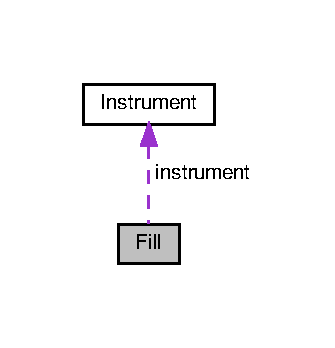
\includegraphics[width=161pt]{classFill__coll__graph}
\end{center}
\end{figure}
\subsection*{Public Types}
\begin{DoxyCompactItemize}
\item 
using \hyperlink{classFill_ab2f91079415160baf6bae4ce4e651882}{Time} = std\+::chrono\+::time\+\_\+point$<$ std\+::chrono\+::system\+\_\+clock $>$
\end{DoxyCompactItemize}
\subsection*{Public Member Functions}
\begin{DoxyCompactItemize}
\item 
\hyperlink{classFill_ac7abcfc5d69d92624d820ac2c54b26a9}{Fill} (const \hyperlink{classInstrument}{Instrument} \&instr, const \hyperlink{classFill_ab2f91079415160baf6bae4ce4e651882}{Time} \&f\+\_\+time, const \hyperlink{fill_8h_a0735734beae0a6b094ce815e727eeca0}{Exchange} \&exch, const unsigned int \&qty, const \hyperlink{fill_8h_a224b9163917ac32fc95a60d8c1eec3aa}{Direction} \&dir, const double \&o\+Price, const double \&e\+Price, const unsigned int \&o\+\_\+id)
\begin{DoxyCompactList}\small\item\em ctor \end{DoxyCompactList}\item 
double \hyperlink{classFill_afc13ac8bde0a76cb798f5fc9a62014fd}{get\+Slippage} () const
\begin{DoxyCompactList}\small\item\em gets the slippage \end{DoxyCompactList}\end{DoxyCompactItemize}
\subsection*{Public Attributes}
\begin{DoxyCompactItemize}
\item 
const \hyperlink{classInstrument}{Instrument} \hyperlink{classFill_ad8cc2217100d31b29c61554adfae4c89}{instrument}
\item 
const \hyperlink{classFill_ab2f91079415160baf6bae4ce4e651882}{Time} \hyperlink{classFill_a3c16af5c63d428b20e145bdd8aed079c}{fill\+\_\+time}
\item 
const \hyperlink{fill_8h_a0735734beae0a6b094ce815e727eeca0}{Exchange} \hyperlink{classFill_affe8391a70b7231659a2c54d38c449ee}{exchange}
\item 
const unsigned int \hyperlink{classFill_a6a19e54b16e7025f2196e6658acf8976}{quantity}
\item 
const \hyperlink{fill_8h_a224b9163917ac32fc95a60d8c1eec3aa}{Direction} \hyperlink{classFill_ab2451992abc07d5a0a217225bea39d3b}{direction}
\item 
const double \hyperlink{classFill_ac7415e2ba0339c0060d13b4900971f25}{order\+\_\+price}
\item 
const double \hyperlink{classFill_aee5774c287161b4b453d688fd75d24af}{execute\+\_\+price}
\item 
const unsigned int \hyperlink{classFill_afd7bfe98f2df0ae03a662083b0526ad1}{order\+\_\+id}
\end{DoxyCompactItemize}


\subsection{Member Typedef Documentation}
\mbox{\Hypertarget{classFill_ab2f91079415160baf6bae4ce4e651882}\label{classFill_ab2f91079415160baf6bae4ce4e651882}} 
\index{Fill@{Fill}!Time@{Time}}
\index{Time@{Time}!Fill@{Fill}}
\subsubsection{\texorpdfstring{Time}{Time}}
{\footnotesize\ttfamily using \hyperlink{classFill_ab2f91079415160baf6bae4ce4e651882}{Fill\+::\+Time} =  std\+::chrono\+::time\+\_\+point$<$std\+::chrono\+::system\+\_\+clock$>$}



\subsection{Constructor \& Destructor Documentation}
\mbox{\Hypertarget{classFill_ac7abcfc5d69d92624d820ac2c54b26a9}\label{classFill_ac7abcfc5d69d92624d820ac2c54b26a9}} 
\index{Fill@{Fill}!Fill@{Fill}}
\index{Fill@{Fill}!Fill@{Fill}}
\subsubsection{\texorpdfstring{Fill()}{Fill()}}
{\footnotesize\ttfamily Fill\+::\+Fill (\begin{DoxyParamCaption}\item[{const \hyperlink{classInstrument}{Instrument} \&}]{instr,  }\item[{const \hyperlink{classFill_ab2f91079415160baf6bae4ce4e651882}{Time} \&}]{f\+\_\+time,  }\item[{const \hyperlink{fill_8h_a0735734beae0a6b094ce815e727eeca0}{Exchange} \&}]{exch,  }\item[{const unsigned int \&}]{qty,  }\item[{const \hyperlink{fill_8h_a224b9163917ac32fc95a60d8c1eec3aa}{Direction} \&}]{dir,  }\item[{const double \&}]{o\+Price,  }\item[{const double \&}]{e\+Price,  }\item[{const unsigned int \&}]{o\+\_\+id }\end{DoxyParamCaption})}



ctor 


\begin{DoxyParams}{Parameters}
{\em instr} & an \hyperlink{classInstrument}{Instrument} object \\
\hline
{\em fill\+\_\+time} & time order was filled \\
\hline
{\em exch} & the exchange it was filled on \\
\hline
{\em qty} & the number of shares \\
\hline
{\em dir} & whether they were bought, sold or shorted \\
\hline
{\em o\+Price} & the price on the order. \\
\hline
{\em e\+Price} & the price that was executed \\
\hline
{\em order\+\_\+id} & a unique order id number \\
\hline
\end{DoxyParams}


\subsection{Member Function Documentation}
\mbox{\Hypertarget{classFill_afc13ac8bde0a76cb798f5fc9a62014fd}\label{classFill_afc13ac8bde0a76cb798f5fc9a62014fd}} 
\index{Fill@{Fill}!get\+Slippage@{get\+Slippage}}
\index{get\+Slippage@{get\+Slippage}!Fill@{Fill}}
\subsubsection{\texorpdfstring{get\+Slippage()}{getSlippage()}}
{\footnotesize\ttfamily double Fill\+::get\+Slippage (\begin{DoxyParamCaption}{ }\end{DoxyParamCaption}) const}



gets the slippage 

\begin{DoxyReturn}{Returns}
how much slippage you endured (as a positive number) 
\end{DoxyReturn}


\subsection{Member Data Documentation}
\mbox{\Hypertarget{classFill_ab2451992abc07d5a0a217225bea39d3b}\label{classFill_ab2451992abc07d5a0a217225bea39d3b}} 
\index{Fill@{Fill}!direction@{direction}}
\index{direction@{direction}!Fill@{Fill}}
\subsubsection{\texorpdfstring{direction}{direction}}
{\footnotesize\ttfamily const \hyperlink{fill_8h_a224b9163917ac32fc95a60d8c1eec3aa}{Direction} Fill\+::direction}

\mbox{\Hypertarget{classFill_affe8391a70b7231659a2c54d38c449ee}\label{classFill_affe8391a70b7231659a2c54d38c449ee}} 
\index{Fill@{Fill}!exchange@{exchange}}
\index{exchange@{exchange}!Fill@{Fill}}
\subsubsection{\texorpdfstring{exchange}{exchange}}
{\footnotesize\ttfamily const \hyperlink{fill_8h_a0735734beae0a6b094ce815e727eeca0}{Exchange} Fill\+::exchange}

\mbox{\Hypertarget{classFill_aee5774c287161b4b453d688fd75d24af}\label{classFill_aee5774c287161b4b453d688fd75d24af}} 
\index{Fill@{Fill}!execute\+\_\+price@{execute\+\_\+price}}
\index{execute\+\_\+price@{execute\+\_\+price}!Fill@{Fill}}
\subsubsection{\texorpdfstring{execute\+\_\+price}{execute\_price}}
{\footnotesize\ttfamily const double Fill\+::execute\+\_\+price}

\mbox{\Hypertarget{classFill_a3c16af5c63d428b20e145bdd8aed079c}\label{classFill_a3c16af5c63d428b20e145bdd8aed079c}} 
\index{Fill@{Fill}!fill\+\_\+time@{fill\+\_\+time}}
\index{fill\+\_\+time@{fill\+\_\+time}!Fill@{Fill}}
\subsubsection{\texorpdfstring{fill\+\_\+time}{fill\_time}}
{\footnotesize\ttfamily const \hyperlink{classFill_ab2f91079415160baf6bae4ce4e651882}{Time} Fill\+::fill\+\_\+time}

\mbox{\Hypertarget{classFill_ad8cc2217100d31b29c61554adfae4c89}\label{classFill_ad8cc2217100d31b29c61554adfae4c89}} 
\index{Fill@{Fill}!instrument@{instrument}}
\index{instrument@{instrument}!Fill@{Fill}}
\subsubsection{\texorpdfstring{instrument}{instrument}}
{\footnotesize\ttfamily const \hyperlink{classInstrument}{Instrument} Fill\+::instrument}

\mbox{\Hypertarget{classFill_afd7bfe98f2df0ae03a662083b0526ad1}\label{classFill_afd7bfe98f2df0ae03a662083b0526ad1}} 
\index{Fill@{Fill}!order\+\_\+id@{order\+\_\+id}}
\index{order\+\_\+id@{order\+\_\+id}!Fill@{Fill}}
\subsubsection{\texorpdfstring{order\+\_\+id}{order\_id}}
{\footnotesize\ttfamily const unsigned int Fill\+::order\+\_\+id}

\mbox{\Hypertarget{classFill_ac7415e2ba0339c0060d13b4900971f25}\label{classFill_ac7415e2ba0339c0060d13b4900971f25}} 
\index{Fill@{Fill}!order\+\_\+price@{order\+\_\+price}}
\index{order\+\_\+price@{order\+\_\+price}!Fill@{Fill}}
\subsubsection{\texorpdfstring{order\+\_\+price}{order\_price}}
{\footnotesize\ttfamily const double Fill\+::order\+\_\+price}

\mbox{\Hypertarget{classFill_a6a19e54b16e7025f2196e6658acf8976}\label{classFill_a6a19e54b16e7025f2196e6658acf8976}} 
\index{Fill@{Fill}!quantity@{quantity}}
\index{quantity@{quantity}!Fill@{Fill}}
\subsubsection{\texorpdfstring{quantity}{quantity}}
{\footnotesize\ttfamily const unsigned int Fill\+::quantity}



The documentation for this class was generated from the following file\+:\begin{DoxyCompactItemize}
\item 
include/\hyperlink{fill_8h}{fill.\+h}\end{DoxyCompactItemize}

\hypertarget{classInstrument}{}\section{Instrument Class Reference}
\label{classInstrument}\index{Instrument@{Instrument}}


{\ttfamily \#include $<$instrument.\+h$>$}

\subsection*{Public Member Functions}
\begin{DoxyCompactItemize}
\item 
\hyperlink{classInstrument_af6112f02c5739bd166b78a1734e79b2c}{Instrument} (const std\+::string \&sym)
\begin{DoxyCompactList}\small\item\em Constructs an \hyperlink{classInstrument}{Instrument} with the provided symbol. \end{DoxyCompactList}\item 
bool \hyperlink{classInstrument_a8ffc6368e7b12588e422145f2b659f9e}{operator$<$} (const \hyperlink{classInstrument}{Instrument} \&other) const
\begin{DoxyCompactList}\small\item\em relational operator that orders the ticker symbols \end{DoxyCompactList}\item 
bool \hyperlink{classInstrument_a5fff991d72c20b0def886d743b6ae0b3}{operator==} (const \hyperlink{classInstrument}{Instrument} \&other) const
\begin{DoxyCompactList}\small\item\em equality operator for the ticker symbols \end{DoxyCompactList}\end{DoxyCompactItemize}
\subsection*{Public Attributes}
\begin{DoxyCompactItemize}
\item 
const std\+::string \hyperlink{classInstrument_a4c469c7cf9512a7b23eb1c26d94a0861}{symbol}
\end{DoxyCompactItemize}


\subsection{Detailed Description}
\begin{DoxyAuthor}{Author}
Benjamin 
\end{DoxyAuthor}
\begin{DoxyDate}{Date}
17/05/18 
\end{DoxyDate}


\subsection{Constructor \& Destructor Documentation}
\mbox{\Hypertarget{classInstrument_af6112f02c5739bd166b78a1734e79b2c}\label{classInstrument_af6112f02c5739bd166b78a1734e79b2c}} 
\index{Instrument@{Instrument}!Instrument@{Instrument}}
\index{Instrument@{Instrument}!Instrument@{Instrument}}
\subsubsection{\texorpdfstring{Instrument()}{Instrument()}}
{\footnotesize\ttfamily Instrument\+::\+Instrument (\begin{DoxyParamCaption}\item[{const std\+::string \&}]{sym }\end{DoxyParamCaption})}



Constructs an \hyperlink{classInstrument}{Instrument} with the provided symbol. 


\begin{DoxyParams}{Parameters}
{\em s} & denotes the symbol \\
\hline
\end{DoxyParams}


\subsection{Member Function Documentation}
\mbox{\Hypertarget{classInstrument_a8ffc6368e7b12588e422145f2b659f9e}\label{classInstrument_a8ffc6368e7b12588e422145f2b659f9e}} 
\index{Instrument@{Instrument}!operator$<$@{operator$<$}}
\index{operator$<$@{operator$<$}!Instrument@{Instrument}}
\subsubsection{\texorpdfstring{operator$<$()}{operator<()}}
{\footnotesize\ttfamily bool Instrument\+::operator$<$ (\begin{DoxyParamCaption}\item[{const \hyperlink{classInstrument}{Instrument} \&}]{other }\end{DoxyParamCaption}) const}



relational operator that orders the ticker symbols 


\begin{DoxyParams}{Parameters}
{\em left} & \\
\hline
{\em right} & \\
\hline
\end{DoxyParams}
\mbox{\Hypertarget{classInstrument_a5fff991d72c20b0def886d743b6ae0b3}\label{classInstrument_a5fff991d72c20b0def886d743b6ae0b3}} 
\index{Instrument@{Instrument}!operator==@{operator==}}
\index{operator==@{operator==}!Instrument@{Instrument}}
\subsubsection{\texorpdfstring{operator==()}{operator==()}}
{\footnotesize\ttfamily bool Instrument\+::operator== (\begin{DoxyParamCaption}\item[{const \hyperlink{classInstrument}{Instrument} \&}]{other }\end{DoxyParamCaption}) const}



equality operator for the ticker symbols 


\begin{DoxyParams}{Parameters}
{\em other} & the \hyperlink{classInstrument}{Instrument} object you\textquotesingle{}re comparing to \\
\hline
\end{DoxyParams}


\subsection{Member Data Documentation}
\mbox{\Hypertarget{classInstrument_a4c469c7cf9512a7b23eb1c26d94a0861}\label{classInstrument_a4c469c7cf9512a7b23eb1c26d94a0861}} 
\index{Instrument@{Instrument}!symbol@{symbol}}
\index{symbol@{symbol}!Instrument@{Instrument}}
\subsubsection{\texorpdfstring{symbol}{symbol}}
{\footnotesize\ttfamily const std\+::string Instrument\+::symbol}



The documentation for this class was generated from the following file\+:\begin{DoxyCompactItemize}
\item 
include/\hyperlink{instrument_8h}{instrument.\+h}\end{DoxyCompactItemize}

\hypertarget{classMarketBar}{}\section{Market\+Bar Class Reference}
\label{classMarketBar}\index{Market\+Bar@{Market\+Bar}}


{\ttfamily \#include $<$market\+\_\+bar.\+h$>$}

\subsection*{Public Types}
\begin{DoxyCompactItemize}
\item 
using \hyperlink{classMarketBar_a0d7dabe1fd00e674ef72f54bb1ff9ad0}{Time} = std\+::chrono\+::time\+\_\+point$<$ std\+::chrono\+::system\+\_\+clock $>$
\end{DoxyCompactItemize}
\subsection*{Public Member Functions}
\begin{DoxyCompactItemize}
\item 
\hyperlink{classMarketBar_a547a73fdfc07436f859da36efb4d8809}{Market\+Bar} ()=default
\begin{DoxyCompactList}\small\item\em Default constructor. \end{DoxyCompactList}\item 
\hyperlink{classMarketBar_ad58b9bb40288a36f1cb9839ce120ea30}{Market\+Bar} (const double \&\hyperlink{classMarketBar_a2d0ebff20fd2d65f1b85da9ce7f5a836}{open}, const double \&\hyperlink{classMarketBar_a77bb9fef6fe9ba65f1b0c7cc0e94a6b7}{high}, const double \&\hyperlink{classMarketBar_aa1d4769489e2ce450d7e376fdfcb6ef4}{low}, const double \&\hyperlink{classMarketBar_a74369b5be9dd83b2410e2bc3e50b8437}{close}, const unsigned int \&vol, const \hyperlink{classMarketBar_a0d7dabe1fd00e674ef72f54bb1ff9ad0}{Time} \&close\+\_\+time)
\begin{DoxyCompactList}\small\item\em Constructs a \hyperlink{classMarketBar}{Market\+Bar} from the provided parameters. \end{DoxyCompactList}\item 
\hyperlink{classMarketBar_a50833d5593d6a3a42f9b5f30772dcafc}{Market\+Bar} (const double \&\hyperlink{classMarketBar_a2d0ebff20fd2d65f1b85da9ce7f5a836}{open}, const double \&\hyperlink{classMarketBar_a77bb9fef6fe9ba65f1b0c7cc0e94a6b7}{high}, const double \&\hyperlink{classMarketBar_aa1d4769489e2ce450d7e376fdfcb6ef4}{low}, const double \&\hyperlink{classMarketBar_a74369b5be9dd83b2410e2bc3e50b8437}{close}, const unsigned int \&vol, const std\+::string \&close\+\_\+time, const std\+::string \&format=\char`\"{}\%Y-\/\%m-\/\%d \%H\+:\%M\+:\%S\char`\"{})
\begin{DoxyCompactList}\small\item\em Constructs a \hyperlink{classMarketBar}{Market\+Bar} from the provided parameters. \end{DoxyCompactList}\item 
\hyperlink{classMarketBar}{Market\+Bar} \& \hyperlink{classMarketBar_aa0a4209809deddf5fb61272d405b1ddc}{operator=} (const \hyperlink{classMarketBar}{Market\+Bar} \&other)=default
\begin{DoxyCompactList}\small\item\em default copy assignment operator generated by the compiler \end{DoxyCompactList}\item 
const double \& \hyperlink{classMarketBar_a2d0ebff20fd2d65f1b85da9ce7f5a836}{open} () const
\begin{DoxyCompactList}\small\item\em gets open \end{DoxyCompactList}\item 
const double \& \hyperlink{classMarketBar_a77bb9fef6fe9ba65f1b0c7cc0e94a6b7}{high} () const
\begin{DoxyCompactList}\small\item\em gets open \end{DoxyCompactList}\item 
const double \& \hyperlink{classMarketBar_aa1d4769489e2ce450d7e376fdfcb6ef4}{low} () const
\begin{DoxyCompactList}\small\item\em gets open \end{DoxyCompactList}\item 
const double \& \hyperlink{classMarketBar_a74369b5be9dd83b2410e2bc3e50b8437}{close} () const
\begin{DoxyCompactList}\small\item\em gets open \end{DoxyCompactList}\item 
const \hyperlink{classMarketBar_a0d7dabe1fd00e674ef72f54bb1ff9ad0}{Time} \& \hyperlink{classMarketBar_aa49e0b737dca9bd90d119ed354f091e4}{time} () const
\begin{DoxyCompactList}\small\item\em time getter \end{DoxyCompactList}\end{DoxyCompactItemize}


\subsection{Detailed Description}
\begin{DoxyAuthor}{Author}
Benjamin 
\end{DoxyAuthor}
\begin{DoxyDate}{Date}
17/05/18 
\end{DoxyDate}


\subsection{Member Typedef Documentation}
\mbox{\Hypertarget{classMarketBar_a0d7dabe1fd00e674ef72f54bb1ff9ad0}\label{classMarketBar_a0d7dabe1fd00e674ef72f54bb1ff9ad0}} 
\index{Market\+Bar@{Market\+Bar}!Time@{Time}}
\index{Time@{Time}!Market\+Bar@{Market\+Bar}}
\subsubsection{\texorpdfstring{Time}{Time}}
{\footnotesize\ttfamily using \hyperlink{classMarketBar_a0d7dabe1fd00e674ef72f54bb1ff9ad0}{Market\+Bar\+::\+Time} =  std\+::chrono\+::time\+\_\+point$<$std\+::chrono\+::system\+\_\+clock$>$}



\subsection{Constructor \& Destructor Documentation}
\mbox{\Hypertarget{classMarketBar_a547a73fdfc07436f859da36efb4d8809}\label{classMarketBar_a547a73fdfc07436f859da36efb4d8809}} 
\index{Market\+Bar@{Market\+Bar}!Market\+Bar@{Market\+Bar}}
\index{Market\+Bar@{Market\+Bar}!Market\+Bar@{Market\+Bar}}
\subsubsection{\texorpdfstring{Market\+Bar()}{MarketBar()}\hspace{0.1cm}{\footnotesize\ttfamily [1/3]}}
{\footnotesize\ttfamily Market\+Bar\+::\+Market\+Bar (\begin{DoxyParamCaption}{ }\end{DoxyParamCaption})\hspace{0.3cm}{\ttfamily [default]}}



Default constructor. 

\mbox{\Hypertarget{classMarketBar_ad58b9bb40288a36f1cb9839ce120ea30}\label{classMarketBar_ad58b9bb40288a36f1cb9839ce120ea30}} 
\index{Market\+Bar@{Market\+Bar}!Market\+Bar@{Market\+Bar}}
\index{Market\+Bar@{Market\+Bar}!Market\+Bar@{Market\+Bar}}
\subsubsection{\texorpdfstring{Market\+Bar()}{MarketBar()}\hspace{0.1cm}{\footnotesize\ttfamily [2/3]}}
{\footnotesize\ttfamily Market\+Bar\+::\+Market\+Bar (\begin{DoxyParamCaption}\item[{const double \&}]{open,  }\item[{const double \&}]{high,  }\item[{const double \&}]{low,  }\item[{const double \&}]{close,  }\item[{const unsigned int \&}]{vol,  }\item[{const \hyperlink{classMarketBar_a0d7dabe1fd00e674ef72f54bb1ff9ad0}{Time} \&}]{close\+\_\+time }\end{DoxyParamCaption})}



Constructs a \hyperlink{classMarketBar}{Market\+Bar} from the provided parameters. 


\begin{DoxyParams}{Parameters}
{\em open} & denotes the instrument opening price of the period \\
\hline
{\em high} & denotes the instrument high price during the period \\
\hline
{\em low} & denotes the instrument low price during the period \\
\hline
{\em close} & denotes the instrument closing price of the period \\
\hline
{\em vol} & denotes the instrument volume over the period \\
\hline
{\em close\+\_\+time} & is the time of the close \\
\hline
\end{DoxyParams}
\mbox{\Hypertarget{classMarketBar_a50833d5593d6a3a42f9b5f30772dcafc}\label{classMarketBar_a50833d5593d6a3a42f9b5f30772dcafc}} 
\index{Market\+Bar@{Market\+Bar}!Market\+Bar@{Market\+Bar}}
\index{Market\+Bar@{Market\+Bar}!Market\+Bar@{Market\+Bar}}
\subsubsection{\texorpdfstring{Market\+Bar()}{MarketBar()}\hspace{0.1cm}{\footnotesize\ttfamily [3/3]}}
{\footnotesize\ttfamily Market\+Bar\+::\+Market\+Bar (\begin{DoxyParamCaption}\item[{const double \&}]{open,  }\item[{const double \&}]{high,  }\item[{const double \&}]{low,  }\item[{const double \&}]{close,  }\item[{const unsigned int \&}]{vol,  }\item[{const std\+::string \&}]{close\+\_\+time,  }\item[{const std\+::string \&}]{format = {\ttfamily \char`\"{}\%Y-\/\%m-\/\%d~\%H\+:\%M\+:\%S\char`\"{}} }\end{DoxyParamCaption})}



Constructs a \hyperlink{classMarketBar}{Market\+Bar} from the provided parameters. 


\begin{DoxyParams}{Parameters}
{\em open} & denotes the instrument opening price of the period \\
\hline
{\em high} & denotes the instrument high price during the period \\
\hline
{\em low} & denotes the instrument low price during the period \\
\hline
{\em close} & denotes the instrument closing price of the period \\
\hline
{\em vol} & denotes the instrument volume over the period \\
\hline
{\em close\+\_\+time} & is the time of the close \\
\hline
{\em time} & format is the format of the tiem \\
\hline
\end{DoxyParams}


\subsection{Member Function Documentation}
\mbox{\Hypertarget{classMarketBar_a74369b5be9dd83b2410e2bc3e50b8437}\label{classMarketBar_a74369b5be9dd83b2410e2bc3e50b8437}} 
\index{Market\+Bar@{Market\+Bar}!close@{close}}
\index{close@{close}!Market\+Bar@{Market\+Bar}}
\subsubsection{\texorpdfstring{close()}{close()}}
{\footnotesize\ttfamily const double\& Market\+Bar\+::close (\begin{DoxyParamCaption}{ }\end{DoxyParamCaption}) const}



gets open 

\begin{DoxyReturn}{Returns}
open 
\end{DoxyReturn}
\mbox{\Hypertarget{classMarketBar_a77bb9fef6fe9ba65f1b0c7cc0e94a6b7}\label{classMarketBar_a77bb9fef6fe9ba65f1b0c7cc0e94a6b7}} 
\index{Market\+Bar@{Market\+Bar}!high@{high}}
\index{high@{high}!Market\+Bar@{Market\+Bar}}
\subsubsection{\texorpdfstring{high()}{high()}}
{\footnotesize\ttfamily const double\& Market\+Bar\+::high (\begin{DoxyParamCaption}{ }\end{DoxyParamCaption}) const}



gets open 

\begin{DoxyReturn}{Returns}
open 
\end{DoxyReturn}
\mbox{\Hypertarget{classMarketBar_aa1d4769489e2ce450d7e376fdfcb6ef4}\label{classMarketBar_aa1d4769489e2ce450d7e376fdfcb6ef4}} 
\index{Market\+Bar@{Market\+Bar}!low@{low}}
\index{low@{low}!Market\+Bar@{Market\+Bar}}
\subsubsection{\texorpdfstring{low()}{low()}}
{\footnotesize\ttfamily const double\& Market\+Bar\+::low (\begin{DoxyParamCaption}{ }\end{DoxyParamCaption}) const}



gets open 

\begin{DoxyReturn}{Returns}
open 
\end{DoxyReturn}
\mbox{\Hypertarget{classMarketBar_a2d0ebff20fd2d65f1b85da9ce7f5a836}\label{classMarketBar_a2d0ebff20fd2d65f1b85da9ce7f5a836}} 
\index{Market\+Bar@{Market\+Bar}!open@{open}}
\index{open@{open}!Market\+Bar@{Market\+Bar}}
\subsubsection{\texorpdfstring{open()}{open()}}
{\footnotesize\ttfamily const double\& Market\+Bar\+::open (\begin{DoxyParamCaption}{ }\end{DoxyParamCaption}) const}



gets open 

\begin{DoxyReturn}{Returns}
open 
\end{DoxyReturn}
\mbox{\Hypertarget{classMarketBar_aa0a4209809deddf5fb61272d405b1ddc}\label{classMarketBar_aa0a4209809deddf5fb61272d405b1ddc}} 
\index{Market\+Bar@{Market\+Bar}!operator=@{operator=}}
\index{operator=@{operator=}!Market\+Bar@{Market\+Bar}}
\subsubsection{\texorpdfstring{operator=()}{operator=()}}
{\footnotesize\ttfamily \hyperlink{classMarketBar}{Market\+Bar}\& Market\+Bar\+::operator= (\begin{DoxyParamCaption}\item[{const \hyperlink{classMarketBar}{Market\+Bar} \&}]{other }\end{DoxyParamCaption})\hspace{0.3cm}{\ttfamily [default]}}



default copy assignment operator generated by the compiler 


\begin{DoxyParams}{Parameters}
{\em other,the} & assigner \hyperlink{classMarketBar}{Market\+Bar} object \\
\hline
\end{DoxyParams}
\mbox{\Hypertarget{classMarketBar_aa49e0b737dca9bd90d119ed354f091e4}\label{classMarketBar_aa49e0b737dca9bd90d119ed354f091e4}} 
\index{Market\+Bar@{Market\+Bar}!time@{time}}
\index{time@{time}!Market\+Bar@{Market\+Bar}}
\subsubsection{\texorpdfstring{time()}{time()}}
{\footnotesize\ttfamily const \hyperlink{classMarketBar_a0d7dabe1fd00e674ef72f54bb1ff9ad0}{Time}\& Market\+Bar\+::time (\begin{DoxyParamCaption}{ }\end{DoxyParamCaption}) const}



time getter 

\begin{DoxyReturn}{Returns}
the time 
\end{DoxyReturn}


The documentation for this class was generated from the following file\+:\begin{DoxyCompactItemize}
\item 
include/\hyperlink{market__bar_8h}{market\+\_\+bar.\+h}\end{DoxyCompactItemize}

\hypertarget{classMarketSnapshot}{}\section{Market\+Snapshot Class Reference}
\label{classMarketSnapshot}\index{Market\+Snapshot@{Market\+Snapshot}}


{\ttfamily \#include $<$market\+\_\+snapshot.\+h$>$}

\subsection*{Public Member Functions}
\begin{DoxyCompactItemize}
\item 
\hyperlink{classMarketSnapshot_afb9edf14f6472bfcae695c5f4a46abff}{Market\+Snapshot} ()=default
\begin{DoxyCompactList}\small\item\em default constructor \end{DoxyCompactList}\item 
\hyperlink{classMarketSnapshot_a5e1530204818ffaea1e479d9371e77ae}{Market\+Snapshot} (const std\+::map$<$ \hyperlink{classInstrument}{Instrument}, \hyperlink{classMarketBar}{Market\+Bar} $>$ \&\hyperlink{classMarketSnapshot_ae8ab3cf282daf2c0001c583ead3b3250}{bars})
\begin{DoxyCompactList}\small\item\em Constructs a new \hyperlink{classMarketSnapshot}{Market\+Snapshot} from the provided information. \end{DoxyCompactList}\item 
\hyperlink{classMarketBar_a0d7dabe1fd00e674ef72f54bb1ff9ad0}{Market\+Bar\+::\+Time} \hyperlink{classMarketSnapshot_a4bc2e6b766eff94c43aa5a45282f797f}{time} () const
\begin{DoxyCompactList}\small\item\em gets the time \end{DoxyCompactList}\item 
std\+::map$<$ \hyperlink{classInstrument}{Instrument}, \hyperlink{classMarketBar}{Market\+Bar} $>$ \hyperlink{classMarketSnapshot_ae8ab3cf282daf2c0001c583ead3b3250}{bars} () const
\begin{DoxyCompactList}\small\item\em gets the map of bars \end{DoxyCompactList}\item 
\hyperlink{classMarketBar}{Market\+Bar} \& \hyperlink{classMarketSnapshot_ad8ad2cc84487f9b21d3db3604d2b1590}{operator\mbox{[}$\,$\mbox{]}} (\hyperlink{classInstrument}{Instrument} instr\+\_\+name)
\begin{DoxyCompactList}\small\item\em returns the \hyperlink{classMarketBar}{Market\+Bar} with instrument name {\ttfamily instr\+\_\+name} \end{DoxyCompactList}\item 
\hyperlink{classMarketBar}{Market\+Bar} \& \hyperlink{classMarketSnapshot_a5029cc166d5c7b895686a25feb0c3af4}{operator\mbox{[}$\,$\mbox{]}} (std\+::string instr\+\_\+name)
\begin{DoxyCompactList}\small\item\em returns the \hyperlink{classMarketBar}{Market\+Bar} with the instrument name \textquotesingle{}instr\+\_\+name\textquotesingle{} \end{DoxyCompactList}\end{DoxyCompactItemize}


\subsection{Detailed Description}
\begin{DoxyAuthor}{Author}
Benjamin 
\end{DoxyAuthor}
\begin{DoxyDate}{Date}
22/05/18 
\end{DoxyDate}


\subsection{Constructor \& Destructor Documentation}
\mbox{\Hypertarget{classMarketSnapshot_afb9edf14f6472bfcae695c5f4a46abff}\label{classMarketSnapshot_afb9edf14f6472bfcae695c5f4a46abff}} 
\index{Market\+Snapshot@{Market\+Snapshot}!Market\+Snapshot@{Market\+Snapshot}}
\index{Market\+Snapshot@{Market\+Snapshot}!Market\+Snapshot@{Market\+Snapshot}}
\subsubsection{\texorpdfstring{Market\+Snapshot()}{MarketSnapshot()}\hspace{0.1cm}{\footnotesize\ttfamily [1/2]}}
{\footnotesize\ttfamily Market\+Snapshot\+::\+Market\+Snapshot (\begin{DoxyParamCaption}{ }\end{DoxyParamCaption})\hspace{0.3cm}{\ttfamily [default]}}



default constructor 

\mbox{\Hypertarget{classMarketSnapshot_a5e1530204818ffaea1e479d9371e77ae}\label{classMarketSnapshot_a5e1530204818ffaea1e479d9371e77ae}} 
\index{Market\+Snapshot@{Market\+Snapshot}!Market\+Snapshot@{Market\+Snapshot}}
\index{Market\+Snapshot@{Market\+Snapshot}!Market\+Snapshot@{Market\+Snapshot}}
\subsubsection{\texorpdfstring{Market\+Snapshot()}{MarketSnapshot()}\hspace{0.1cm}{\footnotesize\ttfamily [2/2]}}
{\footnotesize\ttfamily Market\+Snapshot\+::\+Market\+Snapshot (\begin{DoxyParamCaption}\item[{const std\+::map$<$ \hyperlink{classInstrument}{Instrument}, \hyperlink{classMarketBar}{Market\+Bar} $>$ \&}]{bars }\end{DoxyParamCaption})}



Constructs a new \hyperlink{classMarketSnapshot}{Market\+Snapshot} from the provided information. 


\begin{DoxyParams}{Parameters}
{\em bars} & denotes the snapshot market data \\
\hline
\end{DoxyParams}


\subsection{Member Function Documentation}
\mbox{\Hypertarget{classMarketSnapshot_ae8ab3cf282daf2c0001c583ead3b3250}\label{classMarketSnapshot_ae8ab3cf282daf2c0001c583ead3b3250}} 
\index{Market\+Snapshot@{Market\+Snapshot}!bars@{bars}}
\index{bars@{bars}!Market\+Snapshot@{Market\+Snapshot}}
\subsubsection{\texorpdfstring{bars()}{bars()}}
{\footnotesize\ttfamily std\+::map$<$\hyperlink{classInstrument}{Instrument},\hyperlink{classMarketBar}{Market\+Bar}$>$ Market\+Snapshot\+::bars (\begin{DoxyParamCaption}{ }\end{DoxyParamCaption}) const}



gets the map of bars 

\begin{DoxyReturn}{Returns}
the O\+H\+LC bars 
\end{DoxyReturn}
\mbox{\Hypertarget{classMarketSnapshot_ad8ad2cc84487f9b21d3db3604d2b1590}\label{classMarketSnapshot_ad8ad2cc84487f9b21d3db3604d2b1590}} 
\index{Market\+Snapshot@{Market\+Snapshot}!operator\mbox{[}\mbox{]}@{operator[]}}
\index{operator\mbox{[}\mbox{]}@{operator[]}!Market\+Snapshot@{Market\+Snapshot}}
\subsubsection{\texorpdfstring{operator[]()}{operator[]()}\hspace{0.1cm}{\footnotesize\ttfamily [1/2]}}
{\footnotesize\ttfamily \hyperlink{classMarketBar}{Market\+Bar}\& Market\+Snapshot\+::operator\mbox{[}$\,$\mbox{]} (\begin{DoxyParamCaption}\item[{\hyperlink{classInstrument}{Instrument}}]{instr\+\_\+name }\end{DoxyParamCaption})}



returns the \hyperlink{classMarketBar}{Market\+Bar} with instrument name {\ttfamily instr\+\_\+name} 


\begin{DoxyParams}{Parameters}
{\em instr\+\_\+name} & \\
\hline
\end{DoxyParams}
\begin{DoxyReturn}{Returns}
the associated \hyperlink{classMarketBar}{Market\+Bar} item 
\end{DoxyReturn}
\mbox{\Hypertarget{classMarketSnapshot_a5029cc166d5c7b895686a25feb0c3af4}\label{classMarketSnapshot_a5029cc166d5c7b895686a25feb0c3af4}} 
\index{Market\+Snapshot@{Market\+Snapshot}!operator\mbox{[}\mbox{]}@{operator[]}}
\index{operator\mbox{[}\mbox{]}@{operator[]}!Market\+Snapshot@{Market\+Snapshot}}
\subsubsection{\texorpdfstring{operator[]()}{operator[]()}\hspace{0.1cm}{\footnotesize\ttfamily [2/2]}}
{\footnotesize\ttfamily \hyperlink{classMarketBar}{Market\+Bar}\& Market\+Snapshot\+::operator\mbox{[}$\,$\mbox{]} (\begin{DoxyParamCaption}\item[{std\+::string}]{instr\+\_\+name }\end{DoxyParamCaption})}



returns the \hyperlink{classMarketBar}{Market\+Bar} with the instrument name \textquotesingle{}instr\+\_\+name\textquotesingle{} 


\begin{DoxyParams}{Parameters}
{\em instr\+\_\+name} & the name of which instrument/stock \\
\hline
\end{DoxyParams}
\begin{DoxyReturn}{Returns}
the associated \hyperlink{classMarketBar}{Market\+Bar} item 
\end{DoxyReturn}
\mbox{\Hypertarget{classMarketSnapshot_a4bc2e6b766eff94c43aa5a45282f797f}\label{classMarketSnapshot_a4bc2e6b766eff94c43aa5a45282f797f}} 
\index{Market\+Snapshot@{Market\+Snapshot}!time@{time}}
\index{time@{time}!Market\+Snapshot@{Market\+Snapshot}}
\subsubsection{\texorpdfstring{time()}{time()}}
{\footnotesize\ttfamily \hyperlink{classMarketBar_a0d7dabe1fd00e674ef72f54bb1ff9ad0}{Market\+Bar\+::\+Time} Market\+Snapshot\+::time (\begin{DoxyParamCaption}{ }\end{DoxyParamCaption}) const}



gets the time 

\begin{DoxyReturn}{Returns}
time 
\end{DoxyReturn}


The documentation for this class was generated from the following file\+:\begin{DoxyCompactItemize}
\item 
include/\hyperlink{market__snapshot_8h}{market\+\_\+snapshot.\+h}\end{DoxyCompactItemize}

\hypertarget{classMarketSnapshotsMaker}{}\section{Market\+Snapshots\+Maker Class Reference}
\label{classMarketSnapshotsMaker}\index{Market\+Snapshots\+Maker@{Market\+Snapshots\+Maker}}


{\ttfamily \#include $<$data\+\_\+readers.\+h$>$}

\subsection*{Public Member Functions}
\begin{DoxyCompactItemize}
\item 
\hyperlink{classMarketSnapshotsMaker_a54050922d3dd9f554a5d3e4137e1963c}{Market\+Snapshots\+Maker} (const std\+::string \&data\+\_\+directory, std\+::string delimiter)
\begin{DoxyCompactList}\small\item\em alternative ctor. Will read in every file in a directory and try to get the ticker names automatically \end{DoxyCompactList}\item 
\hyperlink{classMarketSnapshotsMaker_a8107a3b92c32118a667b5e86099ecde8}{Market\+Snapshots\+Maker} (std\+::vector$<$ std\+::string $>$ filenames, std\+::string delimiter, std\+::vector$<$ std\+::string $>$ tickers)
\begin{DoxyCompactList}\small\item\em ctor \end{DoxyCompactList}\item 
std\+::vector$<$ \hyperlink{classMarketSnapshot}{Market\+Snapshot} $>$ \hyperlink{classMarketSnapshotsMaker_a1fbc9bc9f9e8c6bb1641211b027f7b0d}{data} () const
\begin{DoxyCompactList}\small\item\em returns data in a useable format \end{DoxyCompactList}\end{DoxyCompactItemize}


\subsection{Detailed Description}
\begin{DoxyAuthor}{Author}
t 
\end{DoxyAuthor}
\begin{DoxyDate}{Date}
04/07/18 
\end{DoxyDate}


\subsection{Constructor \& Destructor Documentation}
\mbox{\Hypertarget{classMarketSnapshotsMaker_a54050922d3dd9f554a5d3e4137e1963c}\label{classMarketSnapshotsMaker_a54050922d3dd9f554a5d3e4137e1963c}} 
\index{Market\+Snapshots\+Maker@{Market\+Snapshots\+Maker}!Market\+Snapshots\+Maker@{Market\+Snapshots\+Maker}}
\index{Market\+Snapshots\+Maker@{Market\+Snapshots\+Maker}!Market\+Snapshots\+Maker@{Market\+Snapshots\+Maker}}
\subsubsection{\texorpdfstring{Market\+Snapshots\+Maker()}{MarketSnapshotsMaker()}\hspace{0.1cm}{\footnotesize\ttfamily [1/2]}}
{\footnotesize\ttfamily Market\+Snapshots\+Maker\+::\+Market\+Snapshots\+Maker (\begin{DoxyParamCaption}\item[{const std\+::string \&}]{data\+\_\+directory,  }\item[{std\+::string}]{delimiter }\end{DoxyParamCaption})}



alternative ctor. Will read in every file in a directory and try to get the ticker names automatically 


\begin{DoxyParams}{Parameters}
{\em data\+\_\+directory} & where the files are...will try to read in all of the files in their \\
\hline
{\em delimiter} & column delimiter \\
\hline
\end{DoxyParams}
\mbox{\Hypertarget{classMarketSnapshotsMaker_a8107a3b92c32118a667b5e86099ecde8}\label{classMarketSnapshotsMaker_a8107a3b92c32118a667b5e86099ecde8}} 
\index{Market\+Snapshots\+Maker@{Market\+Snapshots\+Maker}!Market\+Snapshots\+Maker@{Market\+Snapshots\+Maker}}
\index{Market\+Snapshots\+Maker@{Market\+Snapshots\+Maker}!Market\+Snapshots\+Maker@{Market\+Snapshots\+Maker}}
\subsubsection{\texorpdfstring{Market\+Snapshots\+Maker()}{MarketSnapshotsMaker()}\hspace{0.1cm}{\footnotesize\ttfamily [2/2]}}
{\footnotesize\ttfamily Market\+Snapshots\+Maker\+::\+Market\+Snapshots\+Maker (\begin{DoxyParamCaption}\item[{std\+::vector$<$ std\+::string $>$}]{filenames,  }\item[{std\+::string}]{delimiter,  }\item[{std\+::vector$<$ std\+::string $>$}]{tickers }\end{DoxyParamCaption})}



ctor 


\begin{DoxyParams}{Parameters}
{\em filenames} & the paths to the files you want to read in \\
\hline
{\em delimiter} & the column delimiter \\
\hline
{\em tickers} & the names of the tickers in the same order as the filenames \\
\hline
\end{DoxyParams}


\subsection{Member Function Documentation}
\mbox{\Hypertarget{classMarketSnapshotsMaker_a1fbc9bc9f9e8c6bb1641211b027f7b0d}\label{classMarketSnapshotsMaker_a1fbc9bc9f9e8c6bb1641211b027f7b0d}} 
\index{Market\+Snapshots\+Maker@{Market\+Snapshots\+Maker}!data@{data}}
\index{data@{data}!Market\+Snapshots\+Maker@{Market\+Snapshots\+Maker}}
\subsubsection{\texorpdfstring{data()}{data()}}
{\footnotesize\ttfamily std\+::vector$<$\hyperlink{classMarketSnapshot}{Market\+Snapshot}$>$ Market\+Snapshots\+Maker\+::data (\begin{DoxyParamCaption}{ }\end{DoxyParamCaption}) const}



returns data in a useable format 

\begin{DoxyReturn}{Returns}
a std\+::vector of Market\+Snapshots 
\end{DoxyReturn}


The documentation for this class was generated from the following file\+:\begin{DoxyCompactItemize}
\item 
include/\hyperlink{data__readers_8h}{data\+\_\+readers.\+h}\end{DoxyCompactItemize}

\hypertarget{classModelBank}{}\section{Model\+Bank Class Reference}
\label{classModelBank}\index{Model\+Bank@{Model\+Bank}}


a container of all your models  




{\ttfamily \#include $<$model\+\_\+bank.\+h$>$}

\subsection*{Public Member Functions}
\begin{DoxyCompactItemize}
\item 
\hyperlink{classModelBank_a781d168f7261cf3247cf1e201c181e09}{Model\+Bank} (const std\+::vector$<$ std\+::string $>$ \&ordered\+\_\+tickers, unsigned int pred\+\_\+type=1)
\begin{DoxyCompactList}\small\item\em ctor \end{DoxyCompactList}\item 
void \hyperlink{classModelBank_a504a7a18eab5bfc72f6760136713a70d}{process\+\_\+snapshot} (const \hyperlink{classMarketSnapshot}{Market\+Snapshot} \&ms)
\end{DoxyCompactItemize}
\subsection*{Protected Attributes}
\begin{DoxyCompactItemize}
\item 
std\+::vector$<$ std\+::unique\+\_\+ptr$<$ \hyperlink{classbase__mod}{base\+\_\+mod} $>$ $>$ \hyperlink{classModelBank_afc89ca7d54b80aed8bc12fec3e584bf0}{m\+\_\+all\+\_\+mods}
\end{DoxyCompactItemize}


\subsection{Detailed Description}
a container of all your models 

\begin{DoxyAuthor}{Author}
taylor stores all of your models user needs to subclass this and add models to the container of unique pointers example\+: m\+\_\+all\+\_\+mods.\+push\+\_\+back(std\+::unique\+\_\+ptr$<$mod4$>$(new mod4(param\+\_\+estimates))); for the bayesian model averaging stuff, assumes uniform priors 
\end{DoxyAuthor}


\subsection{Constructor \& Destructor Documentation}
\mbox{\Hypertarget{classModelBank_a781d168f7261cf3247cf1e201c181e09}\label{classModelBank_a781d168f7261cf3247cf1e201c181e09}} 
\index{Model\+Bank@{Model\+Bank}!Model\+Bank@{Model\+Bank}}
\index{Model\+Bank@{Model\+Bank}!Model\+Bank@{Model\+Bank}}
\subsubsection{\texorpdfstring{Model\+Bank()}{ModelBank()}}
{\footnotesize\ttfamily Model\+Bank\+::\+Model\+Bank (\begin{DoxyParamCaption}\item[{const std\+::vector$<$ std\+::string $>$ \&}]{ordered\+\_\+tickers,  }\item[{unsigned int}]{pred\+\_\+type = {\ttfamily 1} }\end{DoxyParamCaption})}



ctor 


\begin{DoxyParams}{Parameters}
{\em the} & tickers you\textquotesingle{}re looking at in order \\
\hline
{\em pred\+\_\+type} & 1 corresponds with the model that has the best posterior, 2 corresponds with an average \\
\hline
\end{DoxyParams}


\subsection{Member Function Documentation}
\mbox{\Hypertarget{classModelBank_a504a7a18eab5bfc72f6760136713a70d}\label{classModelBank_a504a7a18eab5bfc72f6760136713a70d}} 
\index{Model\+Bank@{Model\+Bank}!process\+\_\+snapshot@{process\+\_\+snapshot}}
\index{process\+\_\+snapshot@{process\+\_\+snapshot}!Model\+Bank@{Model\+Bank}}
\subsubsection{\texorpdfstring{process\+\_\+snapshot()}{process\_snapshot()}}
{\footnotesize\ttfamily void Model\+Bank\+::process\+\_\+snapshot (\begin{DoxyParamCaption}\item[{const \hyperlink{classMarketSnapshot}{Market\+Snapshot} \&}]{ms }\end{DoxyParamCaption})}



\subsection{Member Data Documentation}
\mbox{\Hypertarget{classModelBank_afc89ca7d54b80aed8bc12fec3e584bf0}\label{classModelBank_afc89ca7d54b80aed8bc12fec3e584bf0}} 
\index{Model\+Bank@{Model\+Bank}!m\+\_\+all\+\_\+mods@{m\+\_\+all\+\_\+mods}}
\index{m\+\_\+all\+\_\+mods@{m\+\_\+all\+\_\+mods}!Model\+Bank@{Model\+Bank}}
\subsubsection{\texorpdfstring{m\+\_\+all\+\_\+mods}{m\_all\_mods}}
{\footnotesize\ttfamily std\+::vector$<$std\+::unique\+\_\+ptr$<$\hyperlink{classbase__mod}{base\+\_\+mod}$>$ $>$ Model\+Bank\+::m\+\_\+all\+\_\+mods\hspace{0.3cm}{\ttfamily [protected]}}



The documentation for this class was generated from the following file\+:\begin{DoxyCompactItemize}
\item 
include/\hyperlink{model__bank_8h}{model\+\_\+bank.\+h}\end{DoxyCompactItemize}

\hypertarget{classMoveAve}{}\section{Move\+Ave Class Reference}
\label{classMoveAve}\index{Move\+Ave@{Move\+Ave}}


a simple moving average class used to store the most recent model log-\/likelihoods  




{\ttfamily \#include $<$model\+\_\+bank.\+h$>$}

\subsection*{Public Member Functions}
\begin{DoxyCompactItemize}
\item 
\hyperlink{classMoveAve_a7ba3aea659277902e633d1fca06ddc36}{Move\+Ave} ()=delete
\item 
\hyperlink{classMoveAve_a455db6dea545c3bb47fed299740c5031}{Move\+Ave} (const unsigned int \&width)
\begin{DoxyCompactList}\small\item\em ctor \end{DoxyCompactList}\item 
void \hyperlink{classMoveAve_aedeb10294b2e248f27deb43e30b4a1fc}{on\+New\+Data} (const double \&new\+\_\+data)
\begin{DoxyCompactList}\small\item\em takes in a new data point \end{DoxyCompactList}\item 
double \hyperlink{classMoveAve_a5a48674a3d3a2d92baf896d8321cd909}{get\+Current\+Ave} () const
\begin{DoxyCompactList}\small\item\em get the current average value \end{DoxyCompactList}\item 
double \hyperlink{classMoveAve_a8976714955c304bea3149c51e0c8cd95}{get\+Current\+Sum} () const
\begin{DoxyCompactList}\small\item\em get the current sum of all your data \end{DoxyCompactList}\item 
bool \hyperlink{classMoveAve_a2511f0602d9bffdb8ddc8cd31d81ef66}{is\+Full} () const
\end{DoxyCompactItemize}


\subsection{Detailed Description}
a simple moving average class used to store the most recent model log-\/likelihoods 

\begin{DoxyAuthor}{Author}
taylor 
\end{DoxyAuthor}


\subsection{Constructor \& Destructor Documentation}
\mbox{\Hypertarget{classMoveAve_a7ba3aea659277902e633d1fca06ddc36}\label{classMoveAve_a7ba3aea659277902e633d1fca06ddc36}} 
\index{Move\+Ave@{Move\+Ave}!Move\+Ave@{Move\+Ave}}
\index{Move\+Ave@{Move\+Ave}!Move\+Ave@{Move\+Ave}}
\subsubsection{\texorpdfstring{Move\+Ave()}{MoveAve()}\hspace{0.1cm}{\footnotesize\ttfamily [1/2]}}
{\footnotesize\ttfamily Move\+Ave\+::\+Move\+Ave (\begin{DoxyParamCaption}{ }\end{DoxyParamCaption})\hspace{0.3cm}{\ttfamily [delete]}}

\mbox{\Hypertarget{classMoveAve_a455db6dea545c3bb47fed299740c5031}\label{classMoveAve_a455db6dea545c3bb47fed299740c5031}} 
\index{Move\+Ave@{Move\+Ave}!Move\+Ave@{Move\+Ave}}
\index{Move\+Ave@{Move\+Ave}!Move\+Ave@{Move\+Ave}}
\subsubsection{\texorpdfstring{Move\+Ave()}{MoveAve()}\hspace{0.1cm}{\footnotesize\ttfamily [2/2]}}
{\footnotesize\ttfamily Move\+Ave\+::\+Move\+Ave (\begin{DoxyParamCaption}\item[{const unsigned int \&}]{width }\end{DoxyParamCaption})}



ctor 


\begin{DoxyParams}{Parameters}
{\em width} & how many time points do you want to average over \\
\hline
\end{DoxyParams}


\subsection{Member Function Documentation}
\mbox{\Hypertarget{classMoveAve_a5a48674a3d3a2d92baf896d8321cd909}\label{classMoveAve_a5a48674a3d3a2d92baf896d8321cd909}} 
\index{Move\+Ave@{Move\+Ave}!get\+Current\+Ave@{get\+Current\+Ave}}
\index{get\+Current\+Ave@{get\+Current\+Ave}!Move\+Ave@{Move\+Ave}}
\subsubsection{\texorpdfstring{get\+Current\+Ave()}{getCurrentAve()}}
{\footnotesize\ttfamily double Move\+Ave\+::get\+Current\+Ave (\begin{DoxyParamCaption}{ }\end{DoxyParamCaption}) const}



get the current average value 

\begin{DoxyReturn}{Returns}
the current moving average 
\end{DoxyReturn}
\mbox{\Hypertarget{classMoveAve_a8976714955c304bea3149c51e0c8cd95}\label{classMoveAve_a8976714955c304bea3149c51e0c8cd95}} 
\index{Move\+Ave@{Move\+Ave}!get\+Current\+Sum@{get\+Current\+Sum}}
\index{get\+Current\+Sum@{get\+Current\+Sum}!Move\+Ave@{Move\+Ave}}
\subsubsection{\texorpdfstring{get\+Current\+Sum()}{getCurrentSum()}}
{\footnotesize\ttfamily double Move\+Ave\+::get\+Current\+Sum (\begin{DoxyParamCaption}{ }\end{DoxyParamCaption}) const}



get the current sum of all your data 

\begin{DoxyReturn}{Returns}
the sum 
\end{DoxyReturn}
\mbox{\Hypertarget{classMoveAve_a2511f0602d9bffdb8ddc8cd31d81ef66}\label{classMoveAve_a2511f0602d9bffdb8ddc8cd31d81ef66}} 
\index{Move\+Ave@{Move\+Ave}!is\+Full@{is\+Full}}
\index{is\+Full@{is\+Full}!Move\+Ave@{Move\+Ave}}
\subsubsection{\texorpdfstring{is\+Full()}{isFull()}}
{\footnotesize\ttfamily bool Move\+Ave\+::is\+Full (\begin{DoxyParamCaption}{ }\end{DoxyParamCaption}) const}

\mbox{\Hypertarget{classMoveAve_aedeb10294b2e248f27deb43e30b4a1fc}\label{classMoveAve_aedeb10294b2e248f27deb43e30b4a1fc}} 
\index{Move\+Ave@{Move\+Ave}!on\+New\+Data@{on\+New\+Data}}
\index{on\+New\+Data@{on\+New\+Data}!Move\+Ave@{Move\+Ave}}
\subsubsection{\texorpdfstring{on\+New\+Data()}{onNewData()}}
{\footnotesize\ttfamily void Move\+Ave\+::on\+New\+Data (\begin{DoxyParamCaption}\item[{const double \&}]{new\+\_\+data }\end{DoxyParamCaption})}



takes in a new data point 


\begin{DoxyParams}{Parameters}
{\em new\+\_\+data} & the newest datum \\
\hline
\end{DoxyParams}


The documentation for this class was generated from the following file\+:\begin{DoxyCompactItemize}
\item 
include/\hyperlink{model__bank_8h}{model\+\_\+bank.\+h}\end{DoxyCompactItemize}

\hypertarget{classOrder}{}\section{Order Class Reference}
\label{classOrder}\index{Order@{Order}}


{\ttfamily \#include $<$order.\+h$>$}



Collaboration diagram for Order\+:\nopagebreak
\begin{figure}[H]
\begin{center}
\leavevmode
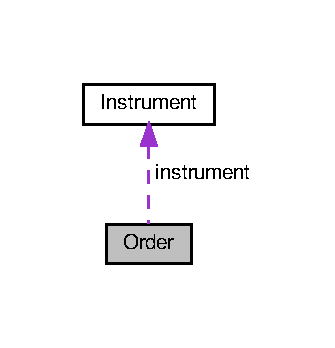
\includegraphics[width=161pt]{classOrder__coll__graph}
\end{center}
\end{figure}
\subsection*{Public Member Functions}
\begin{DoxyCompactItemize}
\item 
\hyperlink{classOrder_a936dad01587c163c6f697c5f3b6406bb}{Order} (const \hyperlink{classInstrument}{Instrument} \&instr, const \hyperlink{order_8h_a57124e387290311f33f3b54a54930418}{Order\+Type} \&order\+\_\+type, const double \&order\+\_\+price, const unsigned int \&qty)
\begin{DoxyCompactList}\small\item\em ctor \end{DoxyCompactList}\end{DoxyCompactItemize}
\subsection*{Public Attributes}
\begin{DoxyCompactItemize}
\item 
const \hyperlink{classInstrument}{Instrument} \hyperlink{classOrder_a34659d82ec58efd7a249c8412be5a8c2}{instrument}
\item 
const \hyperlink{order_8h_a57124e387290311f33f3b54a54930418}{Order\+Type} \hyperlink{classOrder_a131d51d58056d8e34b200b3661d091f2}{type}
\item 
const unsigned int \hyperlink{classOrder_a77525cd65ce276fb5dce2177de41f33f}{quantity}
\item 
double \hyperlink{classOrder_a22df57af82ecda59bd0ed1f7534a170b}{price}
\item 
unsigned int \hyperlink{classOrder_a78c189ccb42636fd4e3e88f6e9d756e4}{id}
\end{DoxyCompactItemize}


\subsection{Detailed Description}
\begin{DoxyAuthor}{Author}
t 
\end{DoxyAuthor}


\subsection{Constructor \& Destructor Documentation}
\mbox{\Hypertarget{classOrder_a936dad01587c163c6f697c5f3b6406bb}\label{classOrder_a936dad01587c163c6f697c5f3b6406bb}} 
\index{Order@{Order}!Order@{Order}}
\index{Order@{Order}!Order@{Order}}
\subsubsection{\texorpdfstring{Order()}{Order()}}
{\footnotesize\ttfamily Order\+::\+Order (\begin{DoxyParamCaption}\item[{const \hyperlink{classInstrument}{Instrument} \&}]{instr,  }\item[{const \hyperlink{order_8h_a57124e387290311f33f3b54a54930418}{Order\+Type} \&}]{order\+\_\+type,  }\item[{const double \&}]{order\+\_\+price,  }\item[{const unsigned int \&}]{qty }\end{DoxyParamCaption})}



ctor 


\begin{DoxyParams}{Parameters}
{\em instr} & the instrument \\
\hline
{\em order\+\_\+type} & the type of order \\
\hline
{\em order\+\_\+price} & the order price (NB\+: if market order, this only is for slippage calc purposes) \\
\hline
{\em qty} & the number of shares \\
\hline
\end{DoxyParams}


\subsection{Member Data Documentation}
\mbox{\Hypertarget{classOrder_a78c189ccb42636fd4e3e88f6e9d756e4}\label{classOrder_a78c189ccb42636fd4e3e88f6e9d756e4}} 
\index{Order@{Order}!id@{id}}
\index{id@{id}!Order@{Order}}
\subsubsection{\texorpdfstring{id}{id}}
{\footnotesize\ttfamily unsigned int Order\+::id}

\mbox{\Hypertarget{classOrder_a34659d82ec58efd7a249c8412be5a8c2}\label{classOrder_a34659d82ec58efd7a249c8412be5a8c2}} 
\index{Order@{Order}!instrument@{instrument}}
\index{instrument@{instrument}!Order@{Order}}
\subsubsection{\texorpdfstring{instrument}{instrument}}
{\footnotesize\ttfamily const \hyperlink{classInstrument}{Instrument} Order\+::instrument}

\mbox{\Hypertarget{classOrder_a22df57af82ecda59bd0ed1f7534a170b}\label{classOrder_a22df57af82ecda59bd0ed1f7534a170b}} 
\index{Order@{Order}!price@{price}}
\index{price@{price}!Order@{Order}}
\subsubsection{\texorpdfstring{price}{price}}
{\footnotesize\ttfamily double Order\+::price}

\mbox{\Hypertarget{classOrder_a77525cd65ce276fb5dce2177de41f33f}\label{classOrder_a77525cd65ce276fb5dce2177de41f33f}} 
\index{Order@{Order}!quantity@{quantity}}
\index{quantity@{quantity}!Order@{Order}}
\subsubsection{\texorpdfstring{quantity}{quantity}}
{\footnotesize\ttfamily const unsigned int Order\+::quantity}

\mbox{\Hypertarget{classOrder_a131d51d58056d8e34b200b3661d091f2}\label{classOrder_a131d51d58056d8e34b200b3661d091f2}} 
\index{Order@{Order}!type@{type}}
\index{type@{type}!Order@{Order}}
\subsubsection{\texorpdfstring{type}{type}}
{\footnotesize\ttfamily const \hyperlink{order_8h_a57124e387290311f33f3b54a54930418}{Order\+Type} Order\+::type}



The documentation for this class was generated from the following file\+:\begin{DoxyCompactItemize}
\item 
include/\hyperlink{order_8h}{order.\+h}\end{DoxyCompactItemize}

\hypertarget{classpnl__calc}{}\section{pnl\+\_\+calc Class Reference}
\label{classpnl__calc}\index{pnl\+\_\+calc@{pnl\+\_\+calc}}


{\ttfamily \#include $<$pnl\+\_\+calculator.\+h$>$}

\subsection*{Public Member Functions}
\begin{DoxyCompactItemize}
\item 
\hyperlink{classpnl__calc_a0b2bc0285a608ec5025b4918f386d18f}{pnl\+\_\+calc} ()
\begin{DoxyCompactList}\small\item\em Default Ctor. Sets everything to 0.\+0. \end{DoxyCompactList}\item 
void \hyperlink{classpnl__calc_a542abad6402d68f140eaecfd1bb845a2}{on\+\_\+fill} (const int \&fill\+\_\+qty, const double \&price, \hyperlink{pnl__calculator_8h_ad733a3c57302a7ac3408d55dc65f2681}{Commission\+Style} cstyle)
\begin{DoxyCompactList}\small\item\em Call this method every time there is a fill. \end{DoxyCompactList}\item 
void \hyperlink{classpnl__calc_aa8fe2e20c0520c17dbba6a37066f2b9c}{on\+\_\+price} (const double \&price)
\begin{DoxyCompactList}\small\item\em Call this method every time there is a market price movement. \end{DoxyCompactList}\item 
const double \& \hyperlink{classpnl__calc_aab99d78b9e204b9a35c559e2f21db16a}{get\+\_\+rpnl} () const
\begin{DoxyCompactList}\small\item\em get the realized pnl \end{DoxyCompactList}\item 
const double \& \hyperlink{classpnl__calc_ab97da4de5a2d1b1c98b055b1256e0109}{get\+\_\+avg\+\_\+price} () const
\begin{DoxyCompactList}\small\item\em get the average price (never negative because cost and qty are always the same sign) \end{DoxyCompactList}\item 
const int \& \hyperlink{classpnl__calc_ae85f96910ab2ca12da816e3d20f69134}{get\+\_\+qty} () const
\begin{DoxyCompactList}\small\item\em get the current quantity of shares owned (or sold if negative) \end{DoxyCompactList}\item 
const \hyperlink{classInstrument}{Instrument} \& \hyperlink{classpnl__calc_a8fae6426142e1318162be3b8177b8e55}{instr} () const
\begin{DoxyCompactList}\small\item\em get the instrument name \end{DoxyCompactList}\item 
const double \& \hyperlink{classpnl__calc_a02d80e8a30ca4d9423961a3600ced266}{get\+\_\+mkt\+\_\+val} () const
\begin{DoxyCompactList}\small\item\em gets the current market-\/value \end{DoxyCompactList}\end{DoxyCompactItemize}


\subsection{Constructor \& Destructor Documentation}
\mbox{\Hypertarget{classpnl__calc_a0b2bc0285a608ec5025b4918f386d18f}\label{classpnl__calc_a0b2bc0285a608ec5025b4918f386d18f}} 
\index{pnl\+\_\+calc@{pnl\+\_\+calc}!pnl\+\_\+calc@{pnl\+\_\+calc}}
\index{pnl\+\_\+calc@{pnl\+\_\+calc}!pnl\+\_\+calc@{pnl\+\_\+calc}}
\subsubsection{\texorpdfstring{pnl\+\_\+calc()}{pnl\_calc()}}
{\footnotesize\ttfamily pnl\+\_\+calc\+::pnl\+\_\+calc (\begin{DoxyParamCaption}{ }\end{DoxyParamCaption})}



Default Ctor. Sets everything to 0.\+0. 



\subsection{Member Function Documentation}
\mbox{\Hypertarget{classpnl__calc_ab97da4de5a2d1b1c98b055b1256e0109}\label{classpnl__calc_ab97da4de5a2d1b1c98b055b1256e0109}} 
\index{pnl\+\_\+calc@{pnl\+\_\+calc}!get\+\_\+avg\+\_\+price@{get\+\_\+avg\+\_\+price}}
\index{get\+\_\+avg\+\_\+price@{get\+\_\+avg\+\_\+price}!pnl\+\_\+calc@{pnl\+\_\+calc}}
\subsubsection{\texorpdfstring{get\+\_\+avg\+\_\+price()}{get\_avg\_price()}}
{\footnotesize\ttfamily const double\& pnl\+\_\+calc\+::get\+\_\+avg\+\_\+price (\begin{DoxyParamCaption}{ }\end{DoxyParamCaption}) const}



get the average price (never negative because cost and qty are always the same sign) 

\begin{DoxyReturn}{Returns}
the average price 
\end{DoxyReturn}
\mbox{\Hypertarget{classpnl__calc_a02d80e8a30ca4d9423961a3600ced266}\label{classpnl__calc_a02d80e8a30ca4d9423961a3600ced266}} 
\index{pnl\+\_\+calc@{pnl\+\_\+calc}!get\+\_\+mkt\+\_\+val@{get\+\_\+mkt\+\_\+val}}
\index{get\+\_\+mkt\+\_\+val@{get\+\_\+mkt\+\_\+val}!pnl\+\_\+calc@{pnl\+\_\+calc}}
\subsubsection{\texorpdfstring{get\+\_\+mkt\+\_\+val()}{get\_mkt\_val()}}
{\footnotesize\ttfamily const double\& pnl\+\_\+calc\+::get\+\_\+mkt\+\_\+val (\begin{DoxyParamCaption}{ }\end{DoxyParamCaption}) const}



gets the current market-\/value 

\begin{DoxyReturn}{Returns}
the current market value 
\end{DoxyReturn}
\mbox{\Hypertarget{classpnl__calc_ae85f96910ab2ca12da816e3d20f69134}\label{classpnl__calc_ae85f96910ab2ca12da816e3d20f69134}} 
\index{pnl\+\_\+calc@{pnl\+\_\+calc}!get\+\_\+qty@{get\+\_\+qty}}
\index{get\+\_\+qty@{get\+\_\+qty}!pnl\+\_\+calc@{pnl\+\_\+calc}}
\subsubsection{\texorpdfstring{get\+\_\+qty()}{get\_qty()}}
{\footnotesize\ttfamily const int\& pnl\+\_\+calc\+::get\+\_\+qty (\begin{DoxyParamCaption}{ }\end{DoxyParamCaption}) const}



get the current quantity of shares owned (or sold if negative) 

\begin{DoxyReturn}{Returns}
the number of shares as an integer 
\end{DoxyReturn}
\mbox{\Hypertarget{classpnl__calc_aab99d78b9e204b9a35c559e2f21db16a}\label{classpnl__calc_aab99d78b9e204b9a35c559e2f21db16a}} 
\index{pnl\+\_\+calc@{pnl\+\_\+calc}!get\+\_\+rpnl@{get\+\_\+rpnl}}
\index{get\+\_\+rpnl@{get\+\_\+rpnl}!pnl\+\_\+calc@{pnl\+\_\+calc}}
\subsubsection{\texorpdfstring{get\+\_\+rpnl()}{get\_rpnl()}}
{\footnotesize\ttfamily const double\& pnl\+\_\+calc\+::get\+\_\+rpnl (\begin{DoxyParamCaption}{ }\end{DoxyParamCaption}) const}



get the realized pnl 

\begin{DoxyReturn}{Returns}
realized pnl 
\end{DoxyReturn}
\mbox{\Hypertarget{classpnl__calc_a8fae6426142e1318162be3b8177b8e55}\label{classpnl__calc_a8fae6426142e1318162be3b8177b8e55}} 
\index{pnl\+\_\+calc@{pnl\+\_\+calc}!instr@{instr}}
\index{instr@{instr}!pnl\+\_\+calc@{pnl\+\_\+calc}}
\subsubsection{\texorpdfstring{instr()}{instr()}}
{\footnotesize\ttfamily const \hyperlink{classInstrument}{Instrument}\& pnl\+\_\+calc\+::instr (\begin{DoxyParamCaption}{ }\end{DoxyParamCaption}) const}



get the instrument name 

\begin{DoxyReturn}{Returns}
the name of the instrument 
\end{DoxyReturn}
\mbox{\Hypertarget{classpnl__calc_a542abad6402d68f140eaecfd1bb845a2}\label{classpnl__calc_a542abad6402d68f140eaecfd1bb845a2}} 
\index{pnl\+\_\+calc@{pnl\+\_\+calc}!on\+\_\+fill@{on\+\_\+fill}}
\index{on\+\_\+fill@{on\+\_\+fill}!pnl\+\_\+calc@{pnl\+\_\+calc}}
\subsubsection{\texorpdfstring{on\+\_\+fill()}{on\_fill()}}
{\footnotesize\ttfamily void pnl\+\_\+calc\+::on\+\_\+fill (\begin{DoxyParamCaption}\item[{const int \&}]{fill\+\_\+qty,  }\item[{const double \&}]{price,  }\item[{\hyperlink{pnl__calculator_8h_ad733a3c57302a7ac3408d55dc65f2681}{Commission\+Style}}]{cstyle }\end{DoxyParamCaption})}



Call this method every time there is a fill. 


\begin{DoxyParams}{Parameters}
{\em fill\+\_\+qty} & signed (negative for sold) amount of shares in the most recent transaction \\
\hline
{\em price} & the price (taken or received) for the transaction \\
\hline
\end{DoxyParams}
\mbox{\Hypertarget{classpnl__calc_aa8fe2e20c0520c17dbba6a37066f2b9c}\label{classpnl__calc_aa8fe2e20c0520c17dbba6a37066f2b9c}} 
\index{pnl\+\_\+calc@{pnl\+\_\+calc}!on\+\_\+price@{on\+\_\+price}}
\index{on\+\_\+price@{on\+\_\+price}!pnl\+\_\+calc@{pnl\+\_\+calc}}
\subsubsection{\texorpdfstring{on\+\_\+price()}{on\_price()}}
{\footnotesize\ttfamily void pnl\+\_\+calc\+::on\+\_\+price (\begin{DoxyParamCaption}\item[{const double \&}]{price }\end{DoxyParamCaption})}



Call this method every time there is a market price movement. 


\begin{DoxyParams}{Parameters}
{\em price} & the most up-\/to-\/date price of an instrument. \\
\hline
\end{DoxyParams}


The documentation for this class was generated from the following file\+:\begin{DoxyCompactItemize}
\item 
include/\hyperlink{pnl__calculator_8h}{pnl\+\_\+calculator.\+h}\end{DoxyCompactItemize}

\hypertarget{classPortfolio}{}\section{Portfolio Class Reference}
\label{classPortfolio}\index{Portfolio@{Portfolio}}


{\ttfamily \#include $<$portfolio.\+h$>$}

\subsection*{Public Member Functions}
\begin{DoxyCompactItemize}
\item 
\hyperlink{classPortfolio_a06e9aac5ff020a789dcdeba2718f11b5}{Portfolio} (double starting\+\_\+cash, std\+::vector$<$ std\+::string $>$ tickers, \hyperlink{pnl__calculator_8h_ad733a3c57302a7ac3408d55dc65f2681}{Commission\+Style} cs=\hyperlink{pnl__calculator_8h_ad733a3c57302a7ac3408d55dc65f2681a4c7c9e42a09b0674cdd86bbbd41b42f3}{Commission\+Style\+::\+I\+B\+Fixed}, bool log=false)
\begin{DoxyCompactList}\small\item\em ctor \end{DoxyCompactList}\item 
void \hyperlink{classPortfolio_aca045221440cf015b8e51f2f4d939745}{read\+All\+Fills} (std\+::queue$<$ \hyperlink{classFill}{Fill} $>$ \&q)
\begin{DoxyCompactList}\small\item\em reads fills from a queue and processes them \end{DoxyCompactList}\item 
void \hyperlink{classPortfolio_aeff3ceffcd454c7479cfef398798f830}{read\+New\+Prices} (\hyperlink{classMarketSnapshot}{Market\+Snapshot} ms)
\begin{DoxyCompactList}\small\item\em processes new market data \end{DoxyCompactList}\item 
Eigen\+::\+Vector\+Xd \hyperlink{classPortfolio_a7a932e1e5b68e8fc8b91d16287f6de30}{get\+Weights1} (const Eigen\+::\+Matrix\+Xd \&Sigma, const Eigen\+::\+Vector\+Xd \&mu, const double \&risk\+Tolerance)
\begin{DoxyCompactList}\small\item\em calculates the weights you need. \end{DoxyCompactList}\item 
void \hyperlink{classPortfolio_a7af1a31a5b6fe1f83c37d8005cc4fd2b}{react\+\_\+and\+\_\+send\+\_\+orders} (Eigen\+::\+Vector\+Xd ideal\+\_\+wts\+\_\+to\+\_\+be, \hyperlink{classExecHandler}{Exec\+Handler} \&order\+\_\+q)
\begin{DoxyCompactList}\small\item\em take in suggested weights from a statistical model for one time period ahead in the future, compute orders, then submit orders to a queue. Also, take the appropriate action if not all conditions are met. \end{DoxyCompactList}\item 
double \hyperlink{classPortfolio_aba2f09887f0859f9407cb961c10f0fef}{get\+Balance} () const
\begin{DoxyCompactList}\small\item\em gets your balance (starting cash plus realized pnls) \end{DoxyCompactList}\item 
double \hyperlink{classPortfolio_aca678d7a74e62ea9fa30843685585b48}{get\+Mkt\+Val} (const std\+::string \&sym) const
\begin{DoxyCompactList}\small\item\em gets the outstanding market value of a position on a given symbol @ \end{DoxyCompactList}\item 
int \hyperlink{classPortfolio_a4362d4cfc98f8cf060e611a74b91673a}{get\+Num\+Shares} (const std\+::string \&sym) const
\begin{DoxyCompactList}\small\item\em gets the number of shares held (negative for short) \end{DoxyCompactList}\end{DoxyCompactItemize}


\subsection{Detailed Description}
\begin{DoxyAuthor}{Author}
t 
\end{DoxyAuthor}
\begin{DoxyDate}{Date}
06/07/18 
\end{DoxyDate}


\subsection{Constructor \& Destructor Documentation}
\mbox{\Hypertarget{classPortfolio_a06e9aac5ff020a789dcdeba2718f11b5}\label{classPortfolio_a06e9aac5ff020a789dcdeba2718f11b5}} 
\index{Portfolio@{Portfolio}!Portfolio@{Portfolio}}
\index{Portfolio@{Portfolio}!Portfolio@{Portfolio}}
\subsubsection{\texorpdfstring{Portfolio()}{Portfolio()}}
{\footnotesize\ttfamily Portfolio\+::\+Portfolio (\begin{DoxyParamCaption}\item[{double}]{starting\+\_\+cash,  }\item[{std\+::vector$<$ std\+::string $>$}]{tickers,  }\item[{\hyperlink{pnl__calculator_8h_ad733a3c57302a7ac3408d55dc65f2681}{Commission\+Style}}]{cs = {\ttfamily \hyperlink{pnl__calculator_8h_ad733a3c57302a7ac3408d55dc65f2681a4c7c9e42a09b0674cdd86bbbd41b42f3}{Commission\+Style\+::\+I\+B\+Fixed}},  }\item[{bool}]{log = {\ttfamily false} }\end{DoxyParamCaption})}



ctor 


\begin{DoxyParams}{Parameters}
{\em starting\+\_\+cash} & \\
\hline
{\em tickers} & all tickers that might have a position on at least once \\
\hline
{\em cs} & commission style \\
\hline
\end{DoxyParams}


\subsection{Member Function Documentation}
\mbox{\Hypertarget{classPortfolio_aba2f09887f0859f9407cb961c10f0fef}\label{classPortfolio_aba2f09887f0859f9407cb961c10f0fef}} 
\index{Portfolio@{Portfolio}!get\+Balance@{get\+Balance}}
\index{get\+Balance@{get\+Balance}!Portfolio@{Portfolio}}
\subsubsection{\texorpdfstring{get\+Balance()}{getBalance()}}
{\footnotesize\ttfamily double Portfolio\+::get\+Balance (\begin{DoxyParamCaption}{ }\end{DoxyParamCaption}) const}



gets your balance (starting cash plus realized pnls) 

\begin{DoxyReturn}{Returns}
the balance in dollars (double) 
\end{DoxyReturn}
\mbox{\Hypertarget{classPortfolio_aca678d7a74e62ea9fa30843685585b48}\label{classPortfolio_aca678d7a74e62ea9fa30843685585b48}} 
\index{Portfolio@{Portfolio}!get\+Mkt\+Val@{get\+Mkt\+Val}}
\index{get\+Mkt\+Val@{get\+Mkt\+Val}!Portfolio@{Portfolio}}
\subsubsection{\texorpdfstring{get\+Mkt\+Val()}{getMktVal()}}
{\footnotesize\ttfamily double Portfolio\+::get\+Mkt\+Val (\begin{DoxyParamCaption}\item[{const std\+::string \&}]{sym }\end{DoxyParamCaption}) const}



gets the outstanding market value of a position on a given symbol @ 

\mbox{\Hypertarget{classPortfolio_a4362d4cfc98f8cf060e611a74b91673a}\label{classPortfolio_a4362d4cfc98f8cf060e611a74b91673a}} 
\index{Portfolio@{Portfolio}!get\+Num\+Shares@{get\+Num\+Shares}}
\index{get\+Num\+Shares@{get\+Num\+Shares}!Portfolio@{Portfolio}}
\subsubsection{\texorpdfstring{get\+Num\+Shares()}{getNumShares()}}
{\footnotesize\ttfamily int Portfolio\+::get\+Num\+Shares (\begin{DoxyParamCaption}\item[{const std\+::string \&}]{sym }\end{DoxyParamCaption}) const}



gets the number of shares held (negative for short) 


\begin{DoxyParams}{Parameters}
{\em sym} & the ticker symbol in all caps \\
\hline
\end{DoxyParams}
\begin{DoxyReturn}{Returns}
the number of shares as int (shares sold are negative) 
\end{DoxyReturn}
\mbox{\Hypertarget{classPortfolio_a7a932e1e5b68e8fc8b91d16287f6de30}\label{classPortfolio_a7a932e1e5b68e8fc8b91d16287f6de30}} 
\index{Portfolio@{Portfolio}!get\+Weights1@{get\+Weights1}}
\index{get\+Weights1@{get\+Weights1}!Portfolio@{Portfolio}}
\subsubsection{\texorpdfstring{get\+Weights1()}{getWeights1()}}
{\footnotesize\ttfamily Eigen\+::\+Vector\+Xd Portfolio\+::get\+Weights1 (\begin{DoxyParamCaption}\item[{const Eigen\+::\+Matrix\+Xd \&}]{Sigma,  }\item[{const Eigen\+::\+Vector\+Xd \&}]{mu,  }\item[{const double \&}]{risk\+Tolerance }\end{DoxyParamCaption})}



calculates the weights you need. 


\begin{DoxyParams}{Parameters}
{\em Sigma} & the positive definite covariance matrix \\
\hline
{\em mu} & the mean returns \\
\hline
{\em risk\+Tolerance} & the nonnegative risk tolerance. must be nonnegative. 0 is the most conservative. \\
\hline
{\em current\+Share\+Prices} & the most up-\/to-\/date share\+Prices \\
\hline
{\em current\+Weights} & the current weights you have \\
\hline
\end{DoxyParams}
\mbox{\Hypertarget{classPortfolio_a7af1a31a5b6fe1f83c37d8005cc4fd2b}\label{classPortfolio_a7af1a31a5b6fe1f83c37d8005cc4fd2b}} 
\index{Portfolio@{Portfolio}!react\+\_\+and\+\_\+send\+\_\+orders@{react\+\_\+and\+\_\+send\+\_\+orders}}
\index{react\+\_\+and\+\_\+send\+\_\+orders@{react\+\_\+and\+\_\+send\+\_\+orders}!Portfolio@{Portfolio}}
\subsubsection{\texorpdfstring{react\+\_\+and\+\_\+send\+\_\+orders()}{react\_and\_send\_orders()}}
{\footnotesize\ttfamily void Portfolio\+::react\+\_\+and\+\_\+send\+\_\+orders (\begin{DoxyParamCaption}\item[{Eigen\+::\+Vector\+Xd}]{ideal\+\_\+wts\+\_\+to\+\_\+be,  }\item[{\hyperlink{classExecHandler}{Exec\+Handler} \&}]{order\+\_\+q }\end{DoxyParamCaption})}



take in suggested weights from a statistical model for one time period ahead in the future, compute orders, then submit orders to a queue. Also, take the appropriate action if not all conditions are met. 


\begin{DoxyParams}{Parameters}
{\em ideal\+\_\+wts\+\_\+to\+\_\+be} & these are based on an optimization procedure (probably) using the mean vector and covariace matrix of the future log returns \\
\hline
{\em order\+\_\+q,the} & order\+\_\+q you submit orders to \\
\hline
\end{DoxyParams}
\mbox{\Hypertarget{classPortfolio_aca045221440cf015b8e51f2f4d939745}\label{classPortfolio_aca045221440cf015b8e51f2f4d939745}} 
\index{Portfolio@{Portfolio}!read\+All\+Fills@{read\+All\+Fills}}
\index{read\+All\+Fills@{read\+All\+Fills}!Portfolio@{Portfolio}}
\subsubsection{\texorpdfstring{read\+All\+Fills()}{readAllFills()}}
{\footnotesize\ttfamily void Portfolio\+::read\+All\+Fills (\begin{DoxyParamCaption}\item[{std\+::queue$<$ \hyperlink{classFill}{Fill} $>$ \&}]{q }\end{DoxyParamCaption})}



reads fills from a queue and processes them 


\begin{DoxyParams}{Parameters}
{\em q} & the queue of fills (passed by non-\/const reference) \\
\hline
\end{DoxyParams}
\mbox{\Hypertarget{classPortfolio_aeff3ceffcd454c7479cfef398798f830}\label{classPortfolio_aeff3ceffcd454c7479cfef398798f830}} 
\index{Portfolio@{Portfolio}!read\+New\+Prices@{read\+New\+Prices}}
\index{read\+New\+Prices@{read\+New\+Prices}!Portfolio@{Portfolio}}
\subsubsection{\texorpdfstring{read\+New\+Prices()}{readNewPrices()}}
{\footnotesize\ttfamily void Portfolio\+::read\+New\+Prices (\begin{DoxyParamCaption}\item[{\hyperlink{classMarketSnapshot}{Market\+Snapshot}}]{ms }\end{DoxyParamCaption})}



processes new market data 


\begin{DoxyParams}{Parameters}
{\em ms} & a market snapshot \\
\hline
\end{DoxyParams}


The documentation for this class was generated from the following file\+:\begin{DoxyCompactItemize}
\item 
include/\hyperlink{portfolio_8h}{portfolio.\+h}\end{DoxyCompactItemize}

\hypertarget{classPositionSummary}{}\section{Position\+Summary Class Reference}
\label{classPositionSummary}\index{Position\+Summary@{Position\+Summary}}


{\ttfamily \#include $<$position\+\_\+summary.\+h$>$}

\subsection*{Public Member Functions}
\begin{DoxyCompactItemize}
\item 
\hyperlink{classPositionSummary_a466b4163900712b20ef0c24661d6fc2f}{Position\+Summary} (double initial\+\_\+capital, const std\+::vector$<$ std\+::string $>$ \&tickers, \hyperlink{pnl__calculator_8h_ad733a3c57302a7ac3408d55dc65f2681}{Commission\+Style} cs)
\begin{DoxyCompactList}\small\item\em sets up a zero position for each symbol \end{DoxyCompactList}\item 
void \hyperlink{classPositionSummary_a4f26c2e4e1776ad2e53ada32d46095e1}{on\+Snapshot} (const \hyperlink{classMarketSnapshot}{Market\+Snapshot} \&ms)
\begin{DoxyCompactList}\small\item\em updates the positions with prices changing. \end{DoxyCompactList}\item 
void \hyperlink{classPositionSummary_a057618b9fbc23598a7353555ff280a44}{on\+Fill} (const \hyperlink{classFill}{Fill} \&fill)
\begin{DoxyCompactList}\small\item\em updates the positions after a fill has been received. \end{DoxyCompactList}\item 
double \hyperlink{classPositionSummary_acb0534c73c95999d2ff2739caedf0773}{get\+Instrument\+Mkt\+Val} (const \hyperlink{classInstrument}{Instrument} \&instr) const
\begin{DoxyCompactList}\small\item\em gets the market value for a particular position. \end{DoxyCompactList}\item 
double \hyperlink{classPositionSummary_a66ed8d8382b50aaca12fd889a2fd6c31}{get\+Instrument\+Mkt\+Val} (const std\+::string \&sym) const
\begin{DoxyCompactList}\small\item\em gets the market value for a particular position \end{DoxyCompactList}\item 
double \hyperlink{classPositionSummary_a1c8772fe401f8d00de795ff09b856d44}{get\+Balance} () const
\begin{DoxyCompactList}\small\item\em gets the current balance (starting cash plus all realized pnls) \end{DoxyCompactList}\end{DoxyCompactItemize}


\subsection{Detailed Description}
\begin{DoxyAuthor}{Author}
t 
\end{DoxyAuthor}
\begin{DoxyDate}{Date}
06/07/18 
\end{DoxyDate}


\subsection{Constructor \& Destructor Documentation}
\mbox{\Hypertarget{classPositionSummary_a466b4163900712b20ef0c24661d6fc2f}\label{classPositionSummary_a466b4163900712b20ef0c24661d6fc2f}} 
\index{Position\+Summary@{Position\+Summary}!Position\+Summary@{Position\+Summary}}
\index{Position\+Summary@{Position\+Summary}!Position\+Summary@{Position\+Summary}}
\subsubsection{\texorpdfstring{Position\+Summary()}{PositionSummary()}}
{\footnotesize\ttfamily Position\+Summary\+::\+Position\+Summary (\begin{DoxyParamCaption}\item[{double}]{initial\+\_\+capital,  }\item[{const std\+::vector$<$ std\+::string $>$ \&}]{tickers,  }\item[{\hyperlink{pnl__calculator_8h_ad733a3c57302a7ac3408d55dc65f2681}{Commission\+Style}}]{cs }\end{DoxyParamCaption})}



sets up a zero position for each symbol 


\begin{DoxyParams}{Parameters}
{\em tickers,the} & ordered collection of which stocks you want to keep track of \\
\hline
\end{DoxyParams}


\subsection{Member Function Documentation}
\mbox{\Hypertarget{classPositionSummary_a1c8772fe401f8d00de795ff09b856d44}\label{classPositionSummary_a1c8772fe401f8d00de795ff09b856d44}} 
\index{Position\+Summary@{Position\+Summary}!get\+Balance@{get\+Balance}}
\index{get\+Balance@{get\+Balance}!Position\+Summary@{Position\+Summary}}
\subsubsection{\texorpdfstring{get\+Balance()}{getBalance()}}
{\footnotesize\ttfamily double Position\+Summary\+::get\+Balance (\begin{DoxyParamCaption}{ }\end{DoxyParamCaption}) const}



gets the current balance (starting cash plus all realized pnls) 

\begin{DoxyReturn}{Returns}
the balance as a double 
\end{DoxyReturn}
\mbox{\Hypertarget{classPositionSummary_acb0534c73c95999d2ff2739caedf0773}\label{classPositionSummary_acb0534c73c95999d2ff2739caedf0773}} 
\index{Position\+Summary@{Position\+Summary}!get\+Instrument\+Mkt\+Val@{get\+Instrument\+Mkt\+Val}}
\index{get\+Instrument\+Mkt\+Val@{get\+Instrument\+Mkt\+Val}!Position\+Summary@{Position\+Summary}}
\subsubsection{\texorpdfstring{get\+Instrument\+Mkt\+Val()}{getInstrumentMktVal()}\hspace{0.1cm}{\footnotesize\ttfamily [1/2]}}
{\footnotesize\ttfamily double Position\+Summary\+::get\+Instrument\+Mkt\+Val (\begin{DoxyParamCaption}\item[{const \hyperlink{classInstrument}{Instrument} \&}]{instr }\end{DoxyParamCaption}) const}



gets the market value for a particular position. 


\begin{DoxyParams}{Parameters}
{\em instr} & an instrument you\textquotesingle{}re interested in. \\
\hline
\end{DoxyParams}
\begin{DoxyReturn}{Returns}
the current market value for \hyperlink{classInstrument}{Instrument} \char`\"{}instr\char`\"{} 
\end{DoxyReturn}
\mbox{\Hypertarget{classPositionSummary_a66ed8d8382b50aaca12fd889a2fd6c31}\label{classPositionSummary_a66ed8d8382b50aaca12fd889a2fd6c31}} 
\index{Position\+Summary@{Position\+Summary}!get\+Instrument\+Mkt\+Val@{get\+Instrument\+Mkt\+Val}}
\index{get\+Instrument\+Mkt\+Val@{get\+Instrument\+Mkt\+Val}!Position\+Summary@{Position\+Summary}}
\subsubsection{\texorpdfstring{get\+Instrument\+Mkt\+Val()}{getInstrumentMktVal()}\hspace{0.1cm}{\footnotesize\ttfamily [2/2]}}
{\footnotesize\ttfamily double Position\+Summary\+::get\+Instrument\+Mkt\+Val (\begin{DoxyParamCaption}\item[{const std\+::string \&}]{sym }\end{DoxyParamCaption}) const}



gets the market value for a particular position 


\begin{DoxyParams}{Parameters}
{\em a} & std\+::string of the parameter you\textquotesingle{}re interested in \\
\hline
\end{DoxyParams}
\begin{DoxyReturn}{Returns}
the current market value for \hyperlink{classInstrument}{Instrument} \char`\"{}instr\char`\"{} 
\end{DoxyReturn}
\mbox{\Hypertarget{classPositionSummary_a057618b9fbc23598a7353555ff280a44}\label{classPositionSummary_a057618b9fbc23598a7353555ff280a44}} 
\index{Position\+Summary@{Position\+Summary}!on\+Fill@{on\+Fill}}
\index{on\+Fill@{on\+Fill}!Position\+Summary@{Position\+Summary}}
\subsubsection{\texorpdfstring{on\+Fill()}{onFill()}}
{\footnotesize\ttfamily void Position\+Summary\+::on\+Fill (\begin{DoxyParamCaption}\item[{const \hyperlink{classFill}{Fill} \&}]{fill }\end{DoxyParamCaption})}



updates the positions after a fill has been received. 


\begin{DoxyParams}{Parameters}
{\em fill} & a \hyperlink{classFill}{Fill} event \\
\hline
\end{DoxyParams}
\mbox{\Hypertarget{classPositionSummary_a4f26c2e4e1776ad2e53ada32d46095e1}\label{classPositionSummary_a4f26c2e4e1776ad2e53ada32d46095e1}} 
\index{Position\+Summary@{Position\+Summary}!on\+Snapshot@{on\+Snapshot}}
\index{on\+Snapshot@{on\+Snapshot}!Position\+Summary@{Position\+Summary}}
\subsubsection{\texorpdfstring{on\+Snapshot()}{onSnapshot()}}
{\footnotesize\ttfamily void Position\+Summary\+::on\+Snapshot (\begin{DoxyParamCaption}\item[{const \hyperlink{classMarketSnapshot}{Market\+Snapshot} \&}]{ms }\end{DoxyParamCaption})}



updates the positions with prices changing. 


\begin{DoxyParams}{Parameters}
{\em ms} & a market snapshot \\
\hline
\end{DoxyParams}


The documentation for this class was generated from the following file\+:\begin{DoxyCompactItemize}
\item 
include/\hyperlink{position__summary_8h}{position\+\_\+summary.\+h}\end{DoxyCompactItemize}

\chapter{File Documentation}
\hypertarget{data__handlers_8h}{}\section{include/data\+\_\+handlers.h File Reference}
\label{data__handlers_8h}\index{include/data\+\_\+handlers.\+h@{include/data\+\_\+handlers.\+h}}


helps convert \hyperlink{classMarketSnapshot}{Market\+Snapshot} events into Eigen\+::\+Vector\+Xds  


{\ttfamily \#include $<$vector$>$}\newline
{\ttfamily \#include $<$string$>$}\newline
{\ttfamily \#include $<$Eigen/\+Dense$>$}\newline
{\ttfamily \#include \char`\"{}market\+\_\+snapshot.\+h\char`\"{}}\newline
Include dependency graph for data\+\_\+handlers.\+h\+:\nopagebreak
\begin{figure}[H]
\begin{center}
\leavevmode
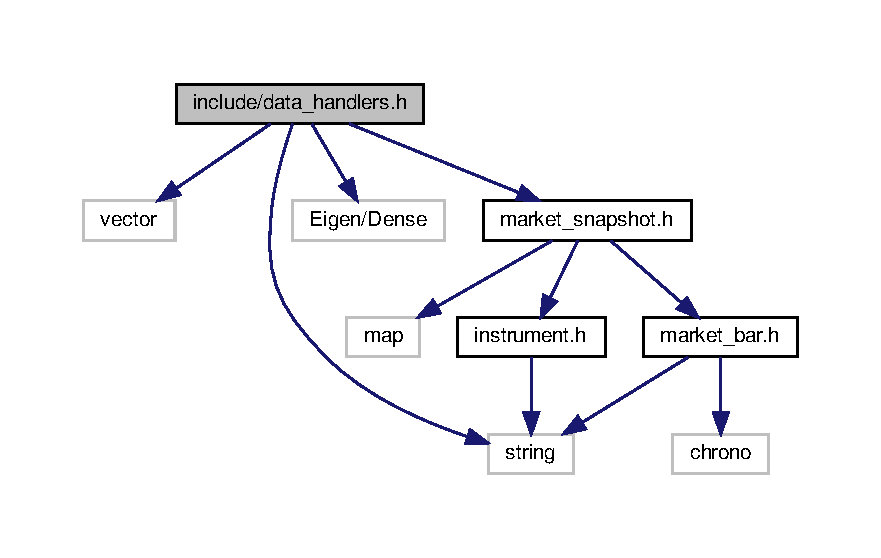
\includegraphics[width=350pt]{data__handlers_8h__incl}
\end{center}
\end{figure}
This graph shows which files directly or indirectly include this file\+:\nopagebreak
\begin{figure}[H]
\begin{center}
\leavevmode
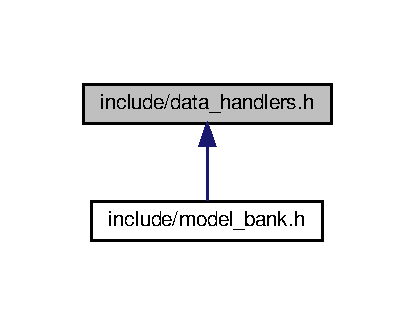
\includegraphics[width=199pt]{data__handlers_8h__dep__incl}
\end{center}
\end{figure}
\subsection*{Classes}
\begin{DoxyCompactItemize}
\item 
class \hyperlink{classDataHandler}{Data\+Handler}
\end{DoxyCompactItemize}


\subsection{Detailed Description}
helps convert \hyperlink{classMarketSnapshot}{Market\+Snapshot} events into Eigen\+::\+Vector\+Xds 


\hypertarget{data__readers_8h}{}\section{include/data\+\_\+readers.h File Reference}
\label{data__readers_8h}\index{include/data\+\_\+readers.\+h@{include/data\+\_\+readers.\+h}}


reads in data (assumed in a certain format), and parses it into a vector of Market\+Snapshots  


{\ttfamily \#include $<$string$>$}\newline
{\ttfamily \#include $<$vector$>$}\newline
{\ttfamily \#include $<$filesystem$>$}\newline
{\ttfamily \#include \char`\"{}market\+\_\+snapshot.\+h\char`\"{}}\newline
Include dependency graph for data\+\_\+readers.\+h\+:\nopagebreak
\begin{figure}[H]
\begin{center}
\leavevmode
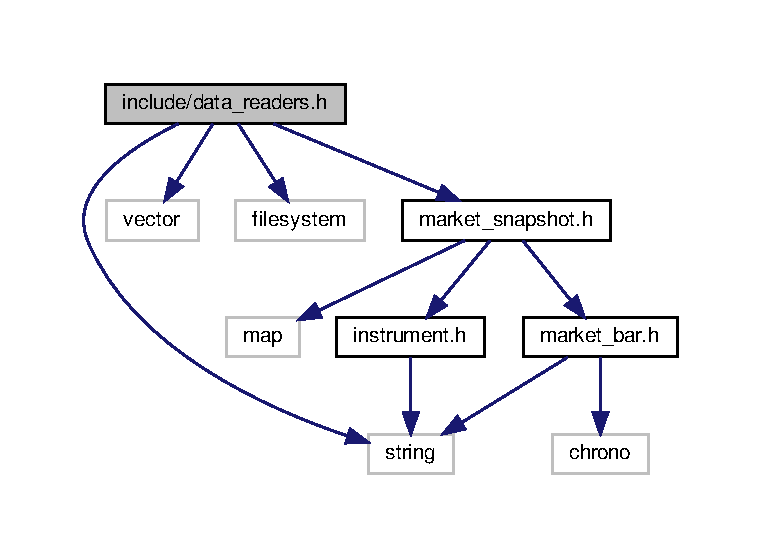
\includegraphics[width=350pt]{data__readers_8h__incl}
\end{center}
\end{figure}
\subsection*{Classes}
\begin{DoxyCompactItemize}
\item 
class \hyperlink{classCSVReader}{C\+S\+V\+Reader}
\item 
class \hyperlink{classMarketSnapshotsMaker}{Market\+Snapshots\+Maker}
\end{DoxyCompactItemize}


\subsection{Detailed Description}
reads in data (assumed in a certain format), and parses it into a vector of Market\+Snapshots 


\hypertarget{execution__handler_8h}{}\section{include/execution\+\_\+handler.h File Reference}
\label{execution__handler_8h}\index{include/execution\+\_\+handler.\+h@{include/execution\+\_\+handler.\+h}}


a glorified std\+::queue. Accepts orders via add\+Order(), and processes them via process\+\_\+orders\+\_\+yield\+\_\+fills().  


{\ttfamily \#include $<$queue$>$}\newline
{\ttfamily \#include $<$iostream$>$}\newline
{\ttfamily \#include \char`\"{}order.\+h\char`\"{}}\newline
{\ttfamily \#include \char`\"{}fill.\+h\char`\"{}}\newline
{\ttfamily \#include \char`\"{}market\+\_\+snapshot.\+h\char`\"{}}\newline
Include dependency graph for execution\+\_\+handler.\+h\+:
\nopagebreak
\begin{figure}[H]
\begin{center}
\leavevmode
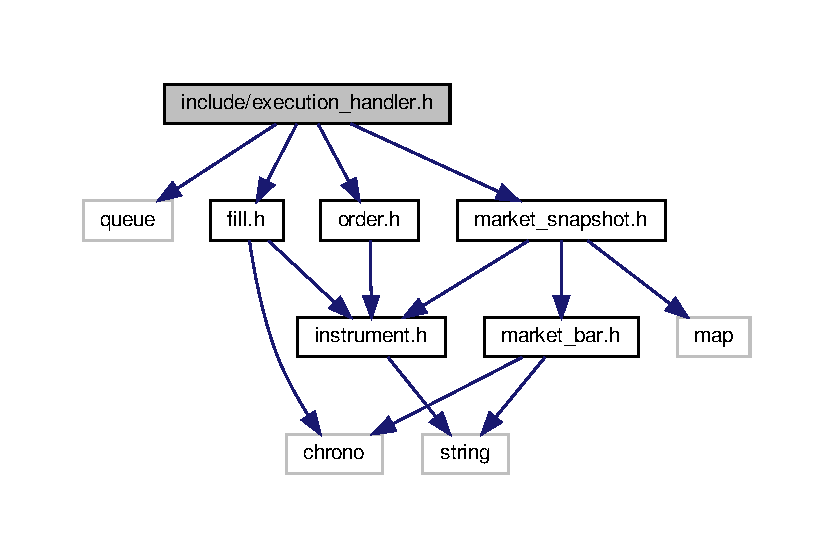
\includegraphics[width=350pt]{execution__handler_8h__incl}
\end{center}
\end{figure}
This graph shows which files directly or indirectly include this file\+:
\nopagebreak
\begin{figure}[H]
\begin{center}
\leavevmode
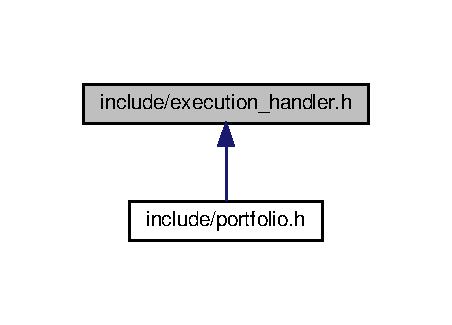
\includegraphics[width=217pt]{execution__handler_8h__dep__incl}
\end{center}
\end{figure}
\subsection*{Classes}
\begin{DoxyCompactItemize}
\item 
class \hyperlink{classExecHandler}{Exec\+Handler}
\end{DoxyCompactItemize}


\subsection{Detailed Description}
a glorified std\+::queue. Accepts orders via add\+Order(), and processes them via process\+\_\+orders\+\_\+yield\+\_\+fills(). 


\hypertarget{fill_8h}{}\section{include/fill.h File Reference}
\label{fill_8h}\index{include/fill.\+h@{include/fill.\+h}}
{\ttfamily \#include $<$chrono$>$}\newline
{\ttfamily \#include \char`\"{}instrument.\+h\char`\"{}}\newline
Include dependency graph for fill.\+h\+:
\nopagebreak
\begin{figure}[H]
\begin{center}
\leavevmode
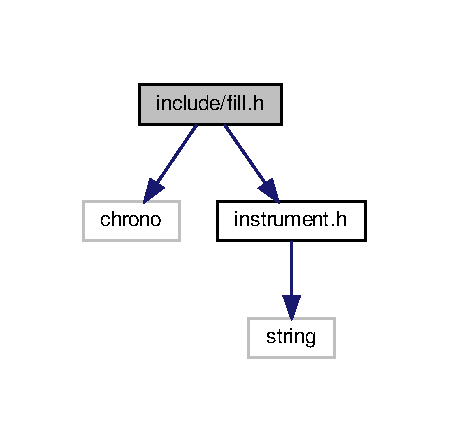
\includegraphics[width=216pt]{fill_8h__incl}
\end{center}
\end{figure}
This graph shows which files directly or indirectly include this file\+:
\nopagebreak
\begin{figure}[H]
\begin{center}
\leavevmode
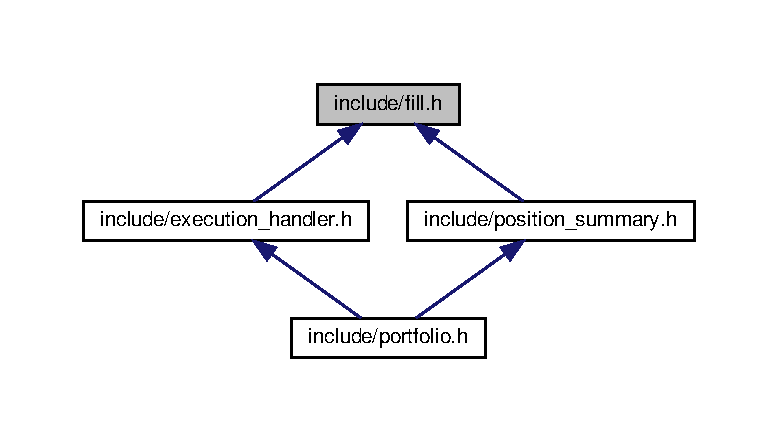
\includegraphics[width=350pt]{fill_8h__dep__incl}
\end{center}
\end{figure}
\subsection*{Classes}
\begin{DoxyCompactItemize}
\item 
class \hyperlink{classFill}{Fill}
\end{DoxyCompactItemize}
\subsection*{Enumerations}
\begin{DoxyCompactItemize}
\item 
enum \hyperlink{fill_8h_a0735734beae0a6b094ce815e727eeca0}{Exchange} \{ \hyperlink{fill_8h_a0735734beae0a6b094ce815e727eeca0af8de4250c89fe3200c8c7126ca364fed}{Exchange\+::\+N\+Y\+SE}, 
\hyperlink{fill_8h_a0735734beae0a6b094ce815e727eeca0a7dfd4a400d092d56e089f4e47411a0a0}{Exchange\+::\+N\+A\+S\+D\+AQ}
 \}
\item 
enum \hyperlink{fill_8h_a224b9163917ac32fc95a60d8c1eec3aa}{Direction} \{ \hyperlink{fill_8h_a224b9163917ac32fc95a60d8c1eec3aaaafe0dd0291140b00bfb1dd459df83933}{Direction\+::\+B\+O\+U\+G\+HT}, 
\hyperlink{fill_8h_a224b9163917ac32fc95a60d8c1eec3aaa8a563f45d976679e363d4e4311706b5b}{Direction\+::\+S\+O\+LD}, 
\hyperlink{fill_8h_a224b9163917ac32fc95a60d8c1eec3aaaa35c2b02966b1563e5bf7b81b8b0cf77}{Direction\+::\+S\+H\+O\+RT}
 \}
\end{DoxyCompactItemize}


\subsection{Enumeration Type Documentation}
\mbox{\Hypertarget{fill_8h_a224b9163917ac32fc95a60d8c1eec3aa}\label{fill_8h_a224b9163917ac32fc95a60d8c1eec3aa}} 
\index{fill.\+h@{fill.\+h}!Direction@{Direction}}
\index{Direction@{Direction}!fill.\+h@{fill.\+h}}
\subsubsection{\texorpdfstring{Direction}{Direction}}
{\footnotesize\ttfamily enum \hyperlink{fill_8h_a224b9163917ac32fc95a60d8c1eec3aa}{Direction}\hspace{0.3cm}{\ttfamily [strong]}}

\begin{DoxyEnumFields}{Enumerator}
\raisebox{\heightof{T}}[0pt][0pt]{\index{B\+O\+U\+G\+HT@{B\+O\+U\+G\+HT}!fill.\+h@{fill.\+h}}\index{fill.\+h@{fill.\+h}!B\+O\+U\+G\+HT@{B\+O\+U\+G\+HT}}}\mbox{\Hypertarget{fill_8h_a224b9163917ac32fc95a60d8c1eec3aaaafe0dd0291140b00bfb1dd459df83933}\label{fill_8h_a224b9163917ac32fc95a60d8c1eec3aaaafe0dd0291140b00bfb1dd459df83933}} 
B\+O\+U\+G\+HT&\\
\hline

\raisebox{\heightof{T}}[0pt][0pt]{\index{S\+O\+LD@{S\+O\+LD}!fill.\+h@{fill.\+h}}\index{fill.\+h@{fill.\+h}!S\+O\+LD@{S\+O\+LD}}}\mbox{\Hypertarget{fill_8h_a224b9163917ac32fc95a60d8c1eec3aaa8a563f45d976679e363d4e4311706b5b}\label{fill_8h_a224b9163917ac32fc95a60d8c1eec3aaa8a563f45d976679e363d4e4311706b5b}} 
S\+O\+LD&\\
\hline

\raisebox{\heightof{T}}[0pt][0pt]{\index{S\+H\+O\+RT@{S\+H\+O\+RT}!fill.\+h@{fill.\+h}}\index{fill.\+h@{fill.\+h}!S\+H\+O\+RT@{S\+H\+O\+RT}}}\mbox{\Hypertarget{fill_8h_a224b9163917ac32fc95a60d8c1eec3aaaa35c2b02966b1563e5bf7b81b8b0cf77}\label{fill_8h_a224b9163917ac32fc95a60d8c1eec3aaaa35c2b02966b1563e5bf7b81b8b0cf77}} 
S\+H\+O\+RT&\\
\hline

\end{DoxyEnumFields}
\mbox{\Hypertarget{fill_8h_a0735734beae0a6b094ce815e727eeca0}\label{fill_8h_a0735734beae0a6b094ce815e727eeca0}} 
\index{fill.\+h@{fill.\+h}!Exchange@{Exchange}}
\index{Exchange@{Exchange}!fill.\+h@{fill.\+h}}
\subsubsection{\texorpdfstring{Exchange}{Exchange}}
{\footnotesize\ttfamily enum \hyperlink{fill_8h_a0735734beae0a6b094ce815e727eeca0}{Exchange}\hspace{0.3cm}{\ttfamily [strong]}}

\begin{DoxyEnumFields}{Enumerator}
\raisebox{\heightof{T}}[0pt][0pt]{\index{N\+Y\+SE@{N\+Y\+SE}!fill.\+h@{fill.\+h}}\index{fill.\+h@{fill.\+h}!N\+Y\+SE@{N\+Y\+SE}}}\mbox{\Hypertarget{fill_8h_a0735734beae0a6b094ce815e727eeca0af8de4250c89fe3200c8c7126ca364fed}\label{fill_8h_a0735734beae0a6b094ce815e727eeca0af8de4250c89fe3200c8c7126ca364fed}} 
N\+Y\+SE&\\
\hline

\raisebox{\heightof{T}}[0pt][0pt]{\index{N\+A\+S\+D\+AQ@{N\+A\+S\+D\+AQ}!fill.\+h@{fill.\+h}}\index{fill.\+h@{fill.\+h}!N\+A\+S\+D\+AQ@{N\+A\+S\+D\+AQ}}}\mbox{\Hypertarget{fill_8h_a0735734beae0a6b094ce815e727eeca0a7dfd4a400d092d56e089f4e47411a0a0}\label{fill_8h_a0735734beae0a6b094ce815e727eeca0a7dfd4a400d092d56e089f4e47411a0a0}} 
N\+A\+S\+D\+AQ&\\
\hline

\end{DoxyEnumFields}

\hypertarget{instrument_8h}{}\section{include/instrument.h File Reference}
\label{instrument_8h}\index{include/instrument.\+h@{include/instrument.\+h}}


Represents a tradable instrument in the financial markets.  


{\ttfamily \#include $<$string$>$}\newline
Include dependency graph for instrument.\+h\+:
\nopagebreak
\begin{figure}[H]
\begin{center}
\leavevmode
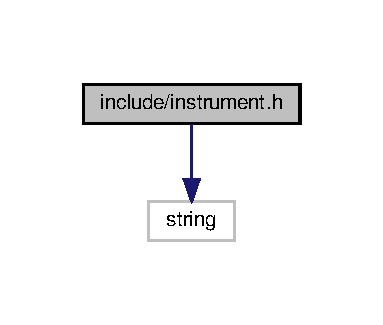
\includegraphics[width=184pt]{instrument_8h__incl}
\end{center}
\end{figure}
This graph shows which files directly or indirectly include this file\+:
\nopagebreak
\begin{figure}[H]
\begin{center}
\leavevmode
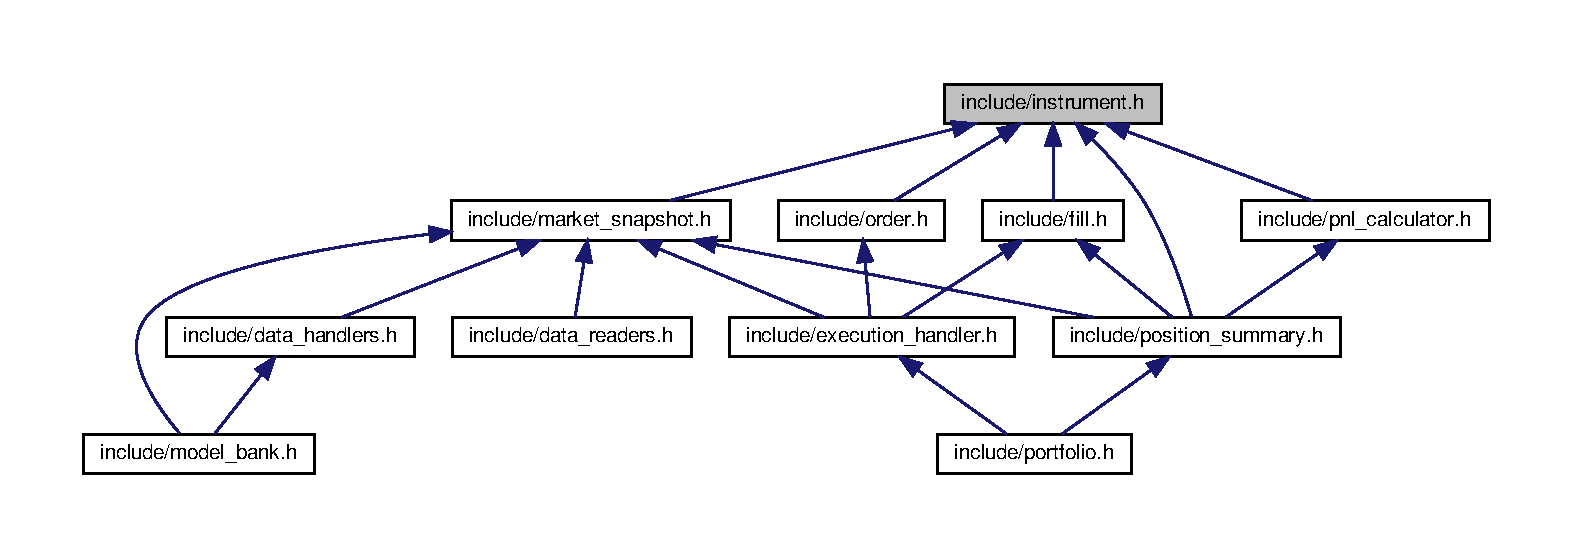
\includegraphics[width=350pt]{instrument_8h__dep__incl}
\end{center}
\end{figure}
\subsection*{Classes}
\begin{DoxyCompactItemize}
\item 
class \hyperlink{classInstrument}{Instrument}
\end{DoxyCompactItemize}


\subsection{Detailed Description}
Represents a tradable instrument in the financial markets. 


\hypertarget{market__bar_8h}{}\section{include/market\+\_\+bar.h File Reference}
\label{market__bar_8h}\index{include/market\+\_\+bar.\+h@{include/market\+\_\+bar.\+h}}


Represents a summary of market data for a particular instrument over a given period of time.  


{\ttfamily \#include $<$chrono$>$}\newline
{\ttfamily \#include $<$string$>$}\newline
Include dependency graph for market\+\_\+bar.\+h\+:
\nopagebreak
\begin{figure}[H]
\begin{center}
\leavevmode
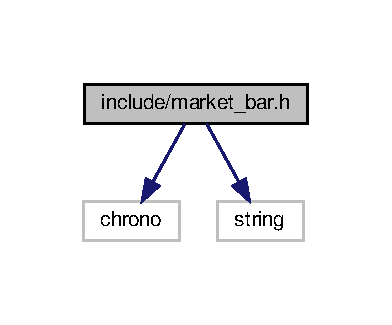
\includegraphics[width=188pt]{market__bar_8h__incl}
\end{center}
\end{figure}
This graph shows which files directly or indirectly include this file\+:
\nopagebreak
\begin{figure}[H]
\begin{center}
\leavevmode
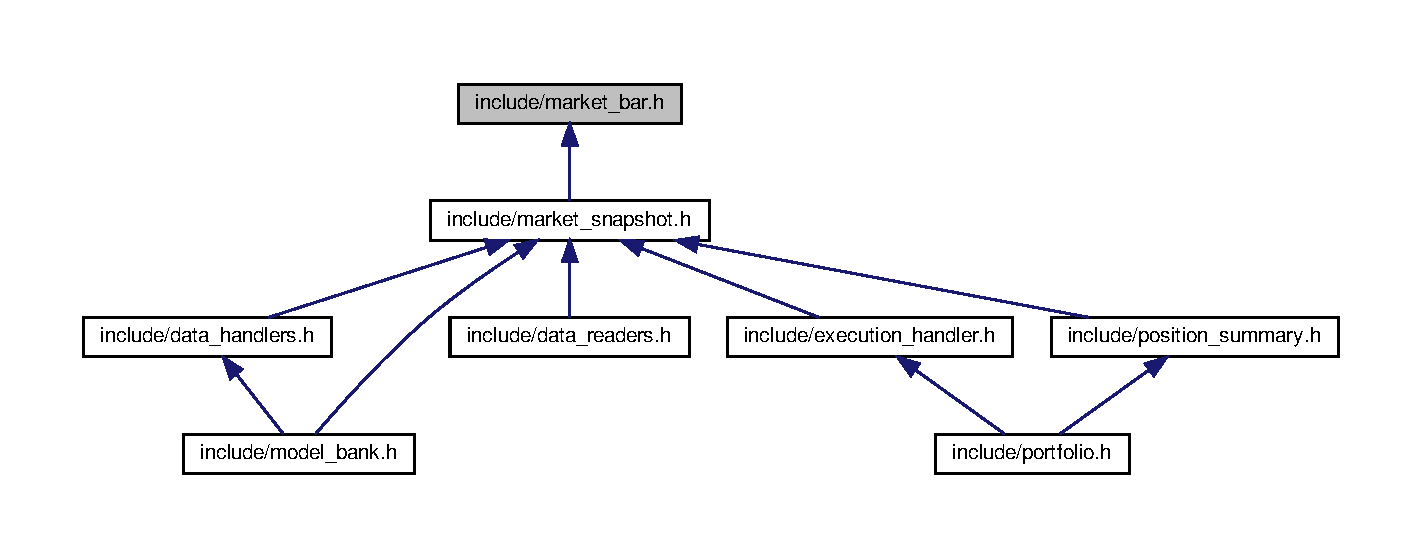
\includegraphics[width=350pt]{market__bar_8h__dep__incl}
\end{center}
\end{figure}
\subsection*{Classes}
\begin{DoxyCompactItemize}
\item 
class \hyperlink{classMarketBar}{Market\+Bar}
\end{DoxyCompactItemize}


\subsection{Detailed Description}
Represents a summary of market data for a particular instrument over a given period of time. 


\hypertarget{market__snapshot_8h}{}\section{include/market\+\_\+snapshot.h File Reference}
\label{market__snapshot_8h}\index{include/market\+\_\+snapshot.\+h@{include/market\+\_\+snapshot.\+h}}


Represents a snapshot of the market at a particular point in time.  


{\ttfamily \#include $<$map$>$}\newline
{\ttfamily \#include \char`\"{}instrument.\+h\char`\"{}}\newline
{\ttfamily \#include \char`\"{}market\+\_\+bar.\+h\char`\"{}}\newline
Include dependency graph for market\+\_\+snapshot.\+h\+:
\nopagebreak
\begin{figure}[H]
\begin{center}
\leavevmode
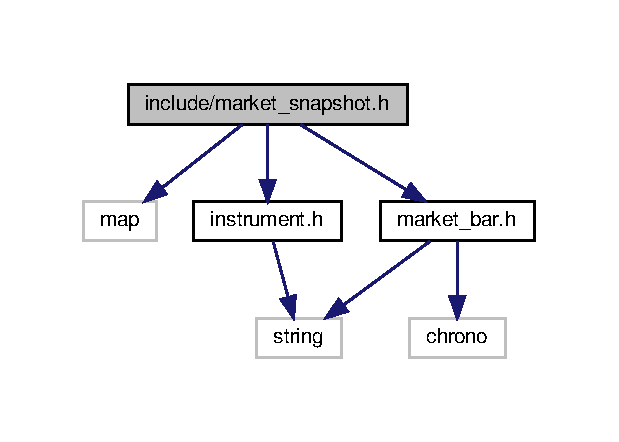
\includegraphics[width=297pt]{market__snapshot_8h__incl}
\end{center}
\end{figure}
This graph shows which files directly or indirectly include this file\+:
\nopagebreak
\begin{figure}[H]
\begin{center}
\leavevmode
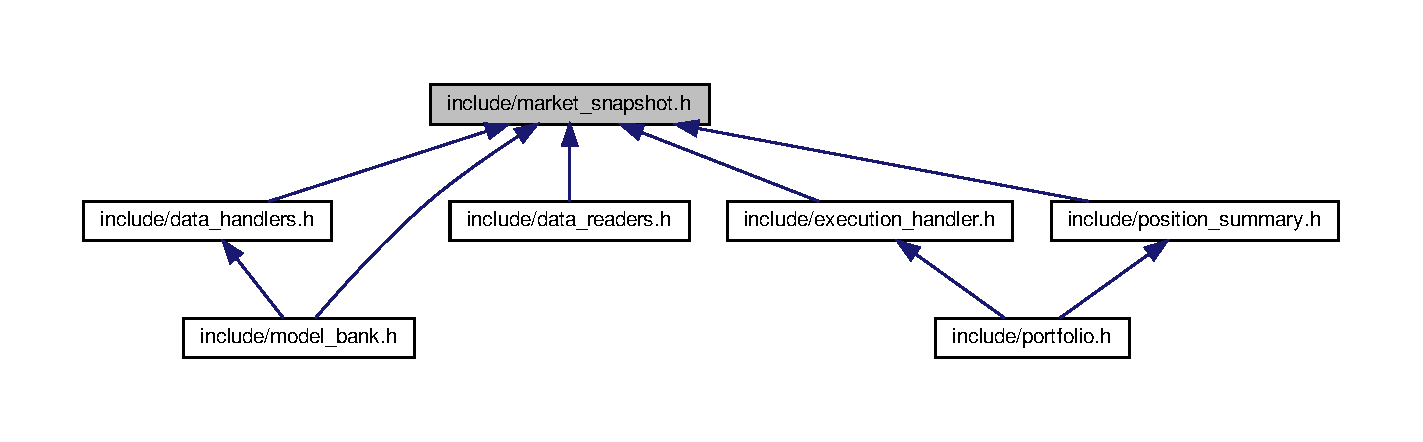
\includegraphics[width=350pt]{market__snapshot_8h__dep__incl}
\end{center}
\end{figure}
\subsection*{Classes}
\begin{DoxyCompactItemize}
\item 
class \hyperlink{classMarketSnapshot}{Market\+Snapshot}
\end{DoxyCompactItemize}


\subsection{Detailed Description}
Represents a snapshot of the market at a particular point in time. 


\hypertarget{model__bank_8h}{}\section{include/model\+\_\+bank.h File Reference}
\label{model__bank_8h}\index{include/model\+\_\+bank.\+h@{include/model\+\_\+bank.\+h}}
{\ttfamily \#include $<$vector$>$}\newline
{\ttfamily \#include $<$string$>$}\newline
{\ttfamily \#include $<$memory$>$}\newline
{\ttfamily \#include \char`\"{}market\+\_\+snapshot.\+h\char`\"{}}\newline
{\ttfamily \#include \char`\"{}data\+\_\+handlers.\+h\char`\"{}}\newline
Include dependency graph for model\+\_\+bank.\+h\+:\nopagebreak
\begin{figure}[H]
\begin{center}
\leavevmode
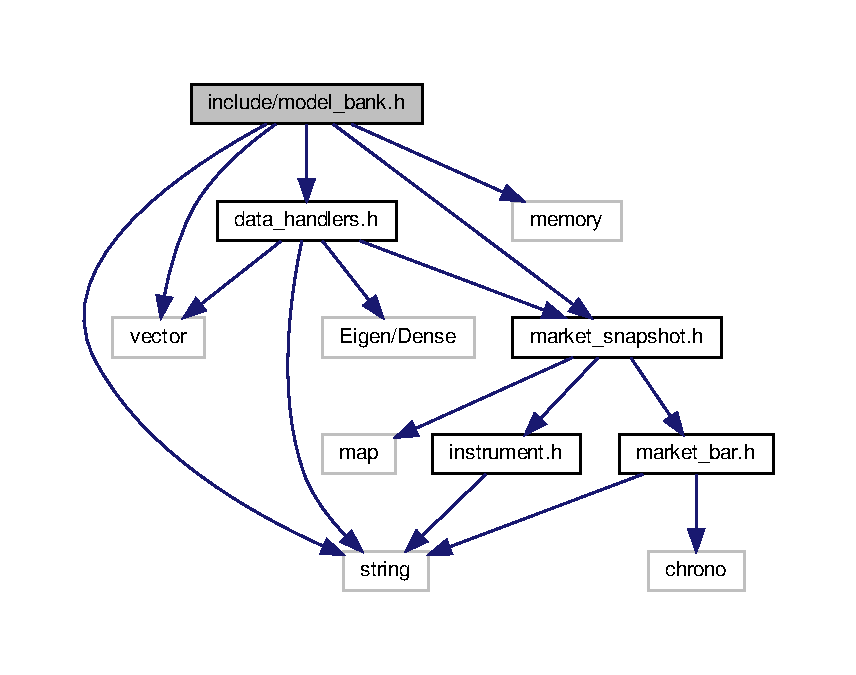
\includegraphics[width=350pt]{model__bank_8h__incl}
\end{center}
\end{figure}
\subsection*{Classes}
\begin{DoxyCompactItemize}
\item 
class \hyperlink{classMoveAve}{Move\+Ave}
\begin{DoxyCompactList}\small\item\em a simple moving average class used to store the most recent model log-\/likelihoods \end{DoxyCompactList}\item 
class \hyperlink{classbase__mod}{base\+\_\+mod}
\begin{DoxyCompactList}\small\item\em each model must inherit from this abstract base class \end{DoxyCompactList}\item 
class \hyperlink{classModelBank}{Model\+Bank}
\begin{DoxyCompactList}\small\item\em a container of all your models \end{DoxyCompactList}\end{DoxyCompactItemize}

\hypertarget{order_8h}{}\section{include/order.h File Reference}
\label{order_8h}\index{include/order.\+h@{include/order.\+h}}


an order class with const public data members  


{\ttfamily \#include \char`\"{}instrument.\+h\char`\"{}}\newline
Include dependency graph for order.\+h\+:
\nopagebreak
\begin{figure}[H]
\begin{center}
\leavevmode
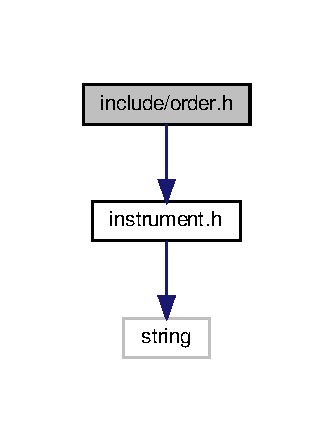
\includegraphics[width=160pt]{order_8h__incl}
\end{center}
\end{figure}
This graph shows which files directly or indirectly include this file\+:
\nopagebreak
\begin{figure}[H]
\begin{center}
\leavevmode
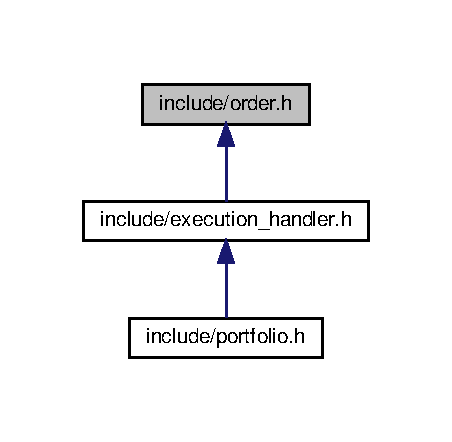
\includegraphics[width=217pt]{order_8h__dep__incl}
\end{center}
\end{figure}
\subsection*{Classes}
\begin{DoxyCompactItemize}
\item 
class \hyperlink{classOrder}{Order}
\end{DoxyCompactItemize}
\subsection*{Enumerations}
\begin{DoxyCompactItemize}
\item 
enum \hyperlink{order_8h_a57124e387290311f33f3b54a54930418}{Order\+Type} \{ \hyperlink{order_8h_a57124e387290311f33f3b54a54930418aab2d3816a4a82987f21ccc6a7af5217e}{Order\+Type\+::market\+Buy}, 
\hyperlink{order_8h_a57124e387290311f33f3b54a54930418a8af2481b23b0ba4afae51e03dcd72c99}{Order\+Type\+::market\+Sell}, 
\hyperlink{order_8h_a57124e387290311f33f3b54a54930418a2343e1f48e543cc7546003cd08b51c90}{Order\+Type\+::limit\+Buy}, 
\hyperlink{order_8h_a57124e387290311f33f3b54a54930418a1b9c1f5993f33853508ff9f10fa3531f}{Order\+Type\+::limit\+Sell}
 \}
\end{DoxyCompactItemize}


\subsection{Detailed Description}
an order class with const public data members 



\subsection{Enumeration Type Documentation}
\mbox{\Hypertarget{order_8h_a57124e387290311f33f3b54a54930418}\label{order_8h_a57124e387290311f33f3b54a54930418}} 
\index{order.\+h@{order.\+h}!Order\+Type@{Order\+Type}}
\index{Order\+Type@{Order\+Type}!order.\+h@{order.\+h}}
\subsubsection{\texorpdfstring{Order\+Type}{OrderType}}
{\footnotesize\ttfamily enum \hyperlink{order_8h_a57124e387290311f33f3b54a54930418}{Order\+Type}\hspace{0.3cm}{\ttfamily [strong]}}

\begin{DoxyEnumFields}{Enumerator}
\raisebox{\heightof{T}}[0pt][0pt]{\index{market\+Buy@{market\+Buy}!order.\+h@{order.\+h}}\index{order.\+h@{order.\+h}!market\+Buy@{market\+Buy}}}\mbox{\Hypertarget{order_8h_a57124e387290311f33f3b54a54930418aab2d3816a4a82987f21ccc6a7af5217e}\label{order_8h_a57124e387290311f33f3b54a54930418aab2d3816a4a82987f21ccc6a7af5217e}} 
market\+Buy&\\
\hline

\raisebox{\heightof{T}}[0pt][0pt]{\index{market\+Sell@{market\+Sell}!order.\+h@{order.\+h}}\index{order.\+h@{order.\+h}!market\+Sell@{market\+Sell}}}\mbox{\Hypertarget{order_8h_a57124e387290311f33f3b54a54930418a8af2481b23b0ba4afae51e03dcd72c99}\label{order_8h_a57124e387290311f33f3b54a54930418a8af2481b23b0ba4afae51e03dcd72c99}} 
market\+Sell&\\
\hline

\raisebox{\heightof{T}}[0pt][0pt]{\index{limit\+Buy@{limit\+Buy}!order.\+h@{order.\+h}}\index{order.\+h@{order.\+h}!limit\+Buy@{limit\+Buy}}}\mbox{\Hypertarget{order_8h_a57124e387290311f33f3b54a54930418a2343e1f48e543cc7546003cd08b51c90}\label{order_8h_a57124e387290311f33f3b54a54930418a2343e1f48e543cc7546003cd08b51c90}} 
limit\+Buy&\\
\hline

\raisebox{\heightof{T}}[0pt][0pt]{\index{limit\+Sell@{limit\+Sell}!order.\+h@{order.\+h}}\index{order.\+h@{order.\+h}!limit\+Sell@{limit\+Sell}}}\mbox{\Hypertarget{order_8h_a57124e387290311f33f3b54a54930418a1b9c1f5993f33853508ff9f10fa3531f}\label{order_8h_a57124e387290311f33f3b54a54930418a1b9c1f5993f33853508ff9f10fa3531f}} 
limit\+Sell&\\
\hline

\end{DoxyEnumFields}

\hypertarget{pnl__calculator_8h}{}\section{include/pnl\+\_\+calculator.h File Reference}
\label{pnl__calculator_8h}\index{include/pnl\+\_\+calculator.\+h@{include/pnl\+\_\+calculator.\+h}}
{\ttfamily \#include \char`\"{}instrument.\+h\char`\"{}}\newline
Include dependency graph for pnl\+\_\+calculator.\+h\+:
\nopagebreak
\begin{figure}[H]
\begin{center}
\leavevmode
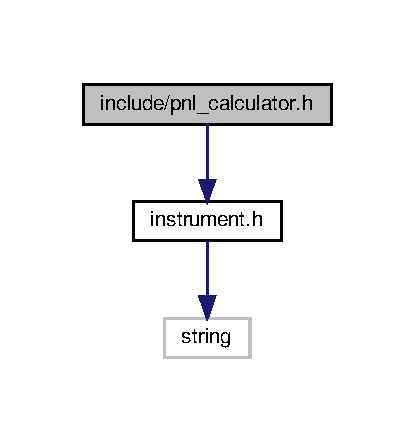
\includegraphics[width=199pt]{pnl__calculator_8h__incl}
\end{center}
\end{figure}
This graph shows which files directly or indirectly include this file\+:
\nopagebreak
\begin{figure}[H]
\begin{center}
\leavevmode
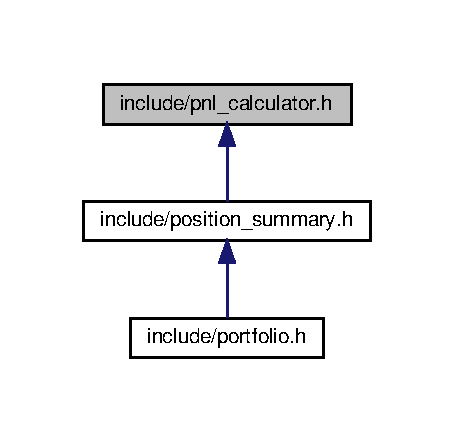
\includegraphics[width=218pt]{pnl__calculator_8h__dep__incl}
\end{center}
\end{figure}
\subsection*{Classes}
\begin{DoxyCompactItemize}
\item 
class \hyperlink{classpnl__calc}{pnl\+\_\+calc}
\end{DoxyCompactItemize}
\subsection*{Enumerations}
\begin{DoxyCompactItemize}
\item 
enum \hyperlink{pnl__calculator_8h_ad733a3c57302a7ac3408d55dc65f2681}{Commission\+Style} \{ \hyperlink{pnl__calculator_8h_ad733a3c57302a7ac3408d55dc65f2681a4c7c9e42a09b0674cdd86bbbd41b42f3}{Commission\+Style\+::\+I\+B\+Fixed}
 \}
\end{DoxyCompactItemize}


\subsection{Enumeration Type Documentation}
\mbox{\Hypertarget{pnl__calculator_8h_ad733a3c57302a7ac3408d55dc65f2681}\label{pnl__calculator_8h_ad733a3c57302a7ac3408d55dc65f2681}} 
\index{pnl\+\_\+calculator.\+h@{pnl\+\_\+calculator.\+h}!Commission\+Style@{Commission\+Style}}
\index{Commission\+Style@{Commission\+Style}!pnl\+\_\+calculator.\+h@{pnl\+\_\+calculator.\+h}}
\subsubsection{\texorpdfstring{Commission\+Style}{CommissionStyle}}
{\footnotesize\ttfamily enum \hyperlink{pnl__calculator_8h_ad733a3c57302a7ac3408d55dc65f2681}{Commission\+Style}\hspace{0.3cm}{\ttfamily [strong]}}

Enum class used for deciding which commission formula. \begin{DoxyEnumFields}{Enumerator}
\raisebox{\heightof{T}}[0pt][0pt]{\index{I\+B\+Fixed@{I\+B\+Fixed}!pnl\+\_\+calculator.\+h@{pnl\+\_\+calculator.\+h}}\index{pnl\+\_\+calculator.\+h@{pnl\+\_\+calculator.\+h}!I\+B\+Fixed@{I\+B\+Fixed}}}\mbox{\Hypertarget{pnl__calculator_8h_ad733a3c57302a7ac3408d55dc65f2681a4c7c9e42a09b0674cdd86bbbd41b42f3}\label{pnl__calculator_8h_ad733a3c57302a7ac3408d55dc65f2681a4c7c9e42a09b0674cdd86bbbd41b42f3}} 
I\+B\+Fixed&\\
\hline

\end{DoxyEnumFields}

\hypertarget{portfolio_8h}{}\section{include/portfolio.h File Reference}
\label{portfolio_8h}\index{include/portfolio.\+h@{include/portfolio.\+h}}


This represents the top level of all accounting details.  


{\ttfamily \#include $<$vector$>$}\newline
{\ttfamily \#include $<$Eigen/\+Dense$>$}\newline
{\ttfamily \#include $<$queue$>$}\newline
{\ttfamily \#include $<$iostream$>$}\newline
{\ttfamily \#include \char`\"{}position\+\_\+summary.\+h\char`\"{}}\newline
{\ttfamily \#include \char`\"{}execution\+\_\+handler.\+h\char`\"{}}\newline
Include dependency graph for portfolio.\+h\+:
\nopagebreak
\begin{figure}[H]
\begin{center}
\leavevmode
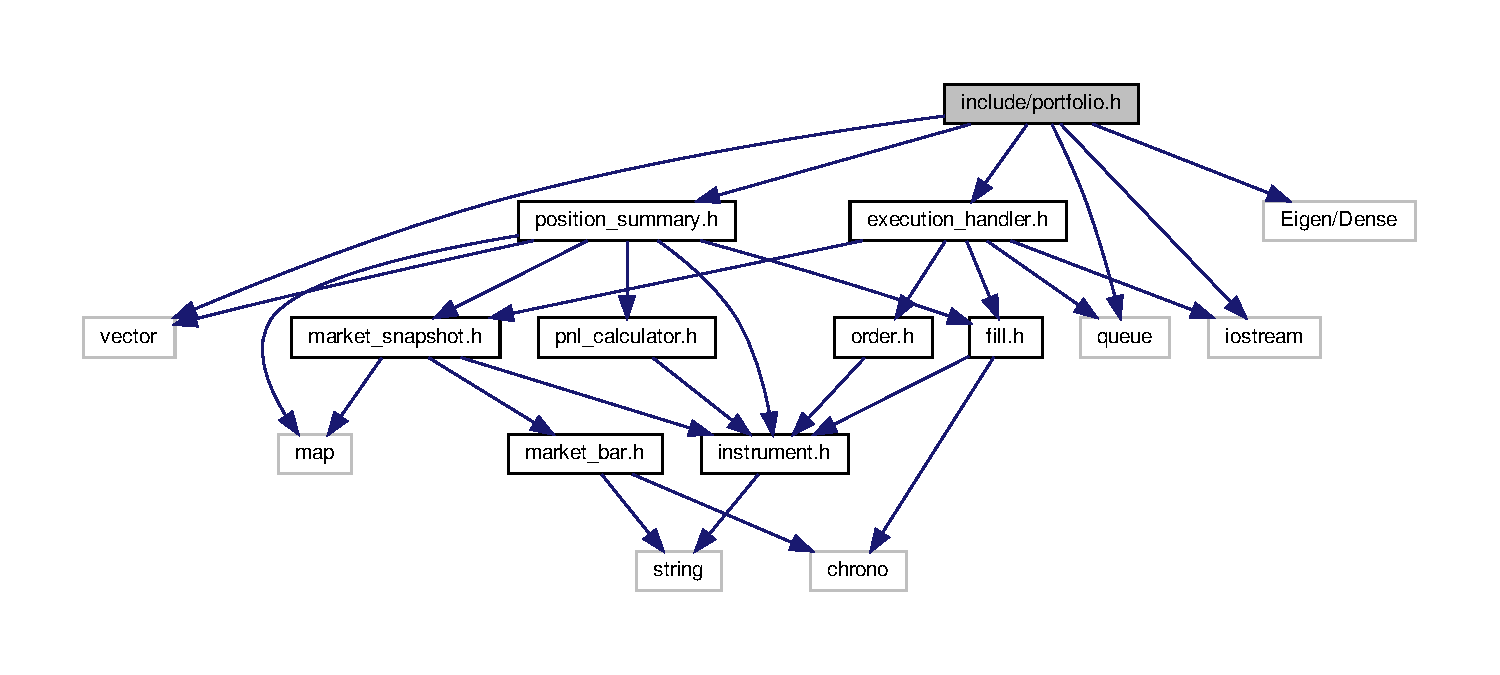
\includegraphics[width=350pt]{portfolio_8h__incl}
\end{center}
\end{figure}
\subsection*{Classes}
\begin{DoxyCompactItemize}
\item 
class \hyperlink{classPortfolio}{Portfolio}
\end{DoxyCompactItemize}


\subsection{Detailed Description}
This represents the top level of all accounting details. 


\begin{DoxyEnumerate}
\item (or 2.) Read all fills and update positions accordingly (read\+All\+Fills)
\item (or 1.) Read in the most recent prices and update positions/info accordingly ( read\+New\+Prices )
\item Receive new ideal weights, calculate orders, and then submit these orders. (update\+On\+New\+Ideal\+Wts) NB\+: this is meant to be subclassed 
\end{DoxyEnumerate}
\hypertarget{position__summary_8h}{}\section{include/position\+\_\+summary.h File Reference}
\label{position__summary_8h}\index{include/position\+\_\+summary.\+h@{include/position\+\_\+summary.\+h}}


Provides a collection of Position objects.  


{\ttfamily \#include $<$map$>$}\newline
{\ttfamily \#include $<$instrument.\+h$>$}\newline
{\ttfamily \#include $<$vector$>$}\newline
{\ttfamily \#include \char`\"{}market\+\_\+snapshot.\+h\char`\"{}}\newline
{\ttfamily \#include \char`\"{}pnl\+\_\+calculator.\+h\char`\"{}}\newline
{\ttfamily \#include \char`\"{}fill.\+h\char`\"{}}\newline
Include dependency graph for position\+\_\+summary.\+h\+:\nopagebreak
\begin{figure}[H]
\begin{center}
\leavevmode
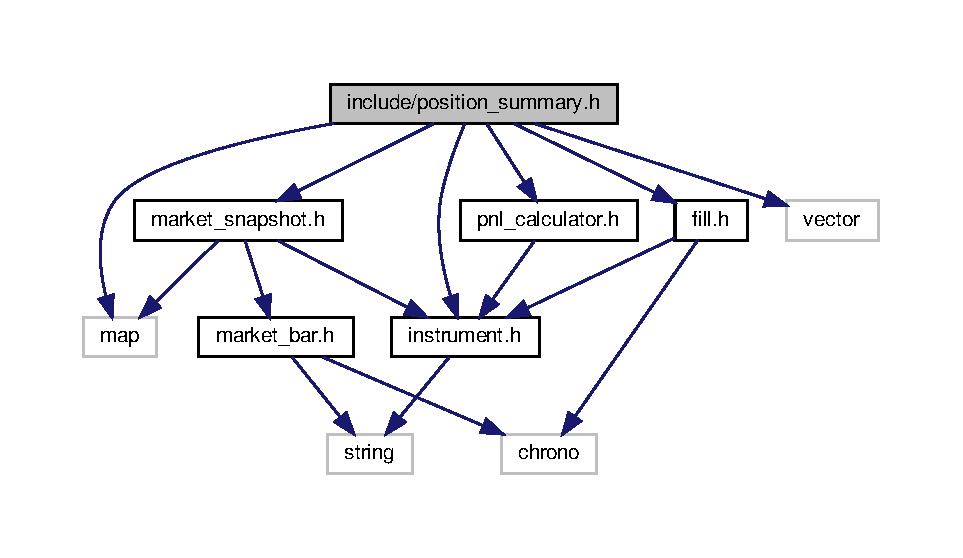
\includegraphics[width=350pt]{position__summary_8h__incl}
\end{center}
\end{figure}
This graph shows which files directly or indirectly include this file\+:\nopagebreak
\begin{figure}[H]
\begin{center}
\leavevmode
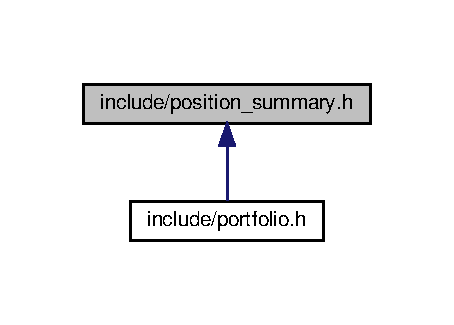
\includegraphics[width=218pt]{position__summary_8h__dep__incl}
\end{center}
\end{figure}
\subsection*{Classes}
\begin{DoxyCompactItemize}
\item 
class \hyperlink{classPositionSummary}{Position\+Summary}
\end{DoxyCompactItemize}


\subsection{Detailed Description}
Provides a collection of Position objects. 


\hypertarget{run__backtest_8h}{}\section{include/run\+\_\+backtest.h File Reference}
\label{run__backtest_8h}\index{include/run\+\_\+backtest.\+h@{include/run\+\_\+backtest.\+h}}

%--- End generated contents ---

% Index
\backmatter
\newpage
\phantomsection
\clearemptydoublepage
\addcontentsline{toc}{chapter}{Index}
\printindex

\end{document}
